%Page layout
\documentclass[12pt, oneside]{report}
\usepackage[T1]{fontenc}
\usepackage[utf8]{inputenc}
\usepackage[a4paper, margin=3cm, top=4cm, bottom=3.5cm, bindingoffset=8mm, headheight=15pt, footskip=35pt]{geometry}
\usepackage{setspace}
\setstretch{1.5}
%\renewcommand{\baselinestretch}{1.5}


%Fonts
\usepackage{lmodern}
%\usepackage{libertine}


%Bibliography
\usepackage[backend=biber, style=authoryear, citestyle=authoryear]{biblatex}
\addbibresource{biblio.bib}



%Quotation marks
\usepackage{dirtytalk}
\usepackage{csquotes}


%Math formulas
\usepackage{amsmath}
\usepackage{amssymb}
\usepackage{amsfonts}
\usepackage{mathtools}
\newtheorem{definition}{Definition}
\newtheorem{theorem}{Theorem}




%Graphs
\usepackage{tikz}
\usetikzlibrary{fit,positioning, arrows, shapes.geometric}


%epigraph in chapter header
\usepackage{epigraph}


%Header
\usepackage{fancyhdr}
\pagestyle{fancy}
\renewcommand{\chaptermark}[1]{\markboth{\fontfamily{qag}\selectfont \chaptername\ \thechapter.\ #1}{}}
\renewcommand{\sectionmark}[1]{\markright{\thesection\ #1}}
%\fancyhead[R]{\fontfamily{qag}\selectfont \leftmark}
%\fancyhead[L]{\fontfamily{qag}\selectfont \rightmark}
%\renewcommand{\footrulewidth}{0.4pt}


%To insert images
\usepackage{graphicx}
\graphicspath{images/}


%General, Sections and Chapters font settings
\usepackage{sectsty}
\sectionfont{\normalfont\scshape\bfseries}
\subsectionfont{\normalfont\scshape\bfseries}
\subsubsectionfont{\normalfont\scshape\bfseries}
\chapterfont{\centering\normalfont\fontfamily{qag}\selectfont}


%References to sections
\usepackage[colorlinks,allcolors=red]{hyperref}
\usepackage{cleveref}
\crefformat{section}{\S#2#1#3}
\crefformat{subsection}{\S#2#1#3}
\crefformat{subsubsection}{\S#2#1#3}


%Detail of the table of content
\setcounter{secnumdepth}{3}
\setcounter{tocdepth}{3}


%Figure caption setup
\usepackage[centerlast]{caption}
\renewcommand{\captionfont}{\linespread{1} \small \slshape \sffamily}
\renewcommand{\captionlabelfont}{\small \bfseries \sffamily}
\setlength{\captionmargin}{1.5cm}


%Title
\title{DRAFT\\Deep Learning: A Statistical Perspective}
\author{Pietro Lesci}
\date{Latest version: 18 January 2019}


%Decoration at the end of chapter
\usepackage{pgfornament}


%Nomenclature
\usepackage{nomencl}
\usepackage{etoolbox}
\makenomenclature


%Plots
\usepackage{pgfplots}
\pgfplotsset{width=10cm,compat=1.9}


%\linespread{1.5}  



%Beginning
\begin{document}

\maketitle


\pagenumbering{roman}%start numbering
\thispagestyle{empty}
\begin{center}
    \vspace*{2.5cm}
    \large
    \textbf{Declaration}
\end{center}
Blank

\clearpage
\thispagestyle{empty}
\begin{center}
    \vspace*{2.5cm}
    \large
    \textbf{Acknowledgment}
\end{center}
Blank

\clearpage
\thispagestyle{empty}
\begin{center}
    \vspace*{2.5cm}
    \large
    \textit{Blank}
\end{center}

\clearpage
\thispagestyle{empty}
\begin{center}
    \vspace*{2.5cm}
    \large
    \textbf{Abstract}
\end{center}
Blank
\clearpage
\tableofcontents
\listoffigures
\pagestyle{plain}

\renewcommand\nomgroup[1]{%
  \bigskip
  \item[\bfseries
  \ifstrequal{#1}{A}{Numbers and Arrays}{%
  \ifstrequal{#1}{B}{Set and Graphs}{%
  \ifstrequal{#1}{C}{Indexing}{%
  \ifstrequal{#1}{D}{Linear Algebra Operations}{%
  \ifstrequal{#1}{E}{Calculus}{%
  \ifstrequal{#1}{F}{Probability and Information Theory}{
  \ifstrequal{#1}{G}{Functions}{%
  \ifstrequal{#1}{H}{Acronyms / Abbreviations}{%
  \ifstrequal{#1}{I}{Datasets and Distributions}{}}}}}}}}}%
]}
\renewcommand{\nomlabel}[1]{\hfil #1\hfil}
\renewcommand{\nomname}{Notation}
\renewcommand{\nompreamble}{The next list describes several symbols that will be later used within the body of the document}



\nomenclature[A]{$x$}{A deterministic quantity, vector or scalar}
\nomenclature[A]{$A$}{A matrix or a random quantity, clarified by the context}
\nomenclature[A]{$W$}{The weight matrix}
\nomenclature[A]{$I$}{Identity matrix}
\nomenclature[A]{$X$}{Training set (matrix with N rows, and D columns)}
\nomenclature[A]{$L$}{Number of layers in the network or per-example loss function, clarified by the context}
\nomenclature[A]{$N_{(test)}$}{Dimensionality of the test set}
\nomenclature[A]{$N$}{Dimensionality of the training set}
\nomenclature[A]{$Q$}{Input dimesionality}
\nomenclature[A]{$D$}{Output dimesionality}

\nomenclature[B]{$\mathbb{R}$}{The set of real numbers}
\nomenclature[B]{$\{0, 1, \dots, n\}$}{The set of all integers between 0 and $n$}

\nomenclature[C]{$a_i$}{Element $i$ of deterministic or random vector $a$, with indexing starting at 1}
\nomenclature[C]{$A_{ij}$}{Element $i,j$ of matrix $A$}
\nomenclature[C]{$A_{i,:}$}{Row $i$ of matrix $A$}
\nomenclature[C]{$A_{:,i}$}{Column $i$ of matrix $A$}

\nomenclature[H]{$i.i.d.$}{Independent and identically distributed}
\nomenclature[H]{DL}{Deep Learning}
\nomenclature[H]{DNN}{Deep Neural Network}


% \renewcommand{\nompostamble}{Throughout the thesis, if not specified otherwise, we denote a generic input variable by the symbol $X$. If $X$ is a vector, its components can be accessed by subscripts $X_d$. A generic output variable is denoted by $Y$.\\
% We use uppercase letters such as $X, Y$ when referring generically to a variable, in the corpus of the text, or to a random variable, in formulae. Observed values are always written in lowercase, hence the $i$th observed value of $X$ is written as $x_i$ (where $x_i$ is again a scalar or vector). \\
% Matrices are always represented by uppercase letters such as $X$; for example, a set of $N$ input vectors of dimension $Q$, $\{x_i\}_{i = 1}^{N}$ would be represented by the $N \times Q$ matrix $X$, also known as \textbf{design matrix}. In general, vectors will not be bold, except when they have $N$ components, that is when they are columns of a design matrix; this convention distinguishes a vector of inputs $x_i$ of dimension $D$ from the $i$th observation from the vector $\mathbf{x}_d$ of dimension $N$ consisting of all the observations on variable $X_D$. All vectors are assumed to be column vectors.\\
% Given this notation we can loosely state the learning task as follows: given the value of an input vector $X$, make a good prediction of the output $Y$, denoted by $\hat{Y}$. Of course, we need data to construct prediction rules, often a lot of it. We thus suppose, henceforth, that we have available a set of measurements $\{(x_i, y_i)\}_{i=1}^{N}$ where $x_i$ is a $D$-dimensional vector of features for object $i$. Sometimes we will use the more explicit indexing of the design matrix: $\mathbf{X}_{i,:} = x_i^\top$ indexing. We refer to $\mathbf{X}$ set as training data; for clarity we may be more explicit with $\mathbf{X}^{(train)}$.
% }

\printnomenclature[3cm]




%\fontfamily{ppl}\selectfont


%blank page
% \newpage\null\thispagestyle{empty}\newpage



%------------------------- Chapter 1 -------------------------
\chapter[Introduction]{Introduction\\Algorithms and Data Models: The Anatomy of Learners}
\pagestyle{fancy}
\pagenumbering{arabic} 


The desire to create machines capable of thinking accompanies the human kind since the first programmable computer was invented. Nowadays, artificial intelligence (AI) is a thriving field of research that encompasses various disciplines such as computer science, engineering, statistics, neuroscience, biology, with applications that range from automating routine labour, interpreting images, understanding speech, to making diagnoses in medicine.

Problems that are intellectually difficult for humans to tackle, namely those problems that can be described by a list of formal, mathematical rules, are among the easiest for computers to solve. The real challenge to AI is the resolution of tasks relatively easy for people to perform, but hard to describe in formal terms -- problems that we, as human beings, solve intuitively, instinctively -- such as recognizing objects in images. This instinctive \say{intuitions} are drawn from experience: collections of small facts (data) and personal judgments of facts (information)\footnote{One research project that aims at producing completely automated analyses and reports is the \textit{Automatic Statistician} [\texttt{https://automaticstatistician.com}]: the current version of the Automatic Statistician is a system which explores an open-ended space of possible statistical models to discover a good explanation of the data, and then produces a detailed report with figures and natural-language text. The system is based on reasoning over an open-ended collection of nonparametric models using Bayesian inference.}.

One solution to let machines mimic the process of deduction from experience is to hard-code the knowledge about the reality in formal language, allowing the computer to reason using logical inference rules. This approach, called \textbf{knowledge-based} [\cite{Goodfellow-et-al-2016}], is brute-force in nature and not viable in many practical applications.

Therefore, AI systems need to have the ability to \say{build} their own knowledge by extracting information from raw data. This field of research is known as \textbf{machine learning}. However, the performance of this approach crucially depends on the \textit{representation} of data used -- the usual maxim \say{garbage in, garbage out}. Each bit of information included in the representation is called \textbf{feature}. Selecting or extracting features, that form representations, from raw data is a form of art of its own. Often, as an alternative to hand-designed features, machine learning algorithms are used to learn such \textit{representations} besides learning the \textit{mapping} from representations to outputs. This approach is called \textbf{representation leaning} [\cite{Goodfellow-et-al-2016}]. 

Regardless the methodology used to build such features, the aim is often to separate the \textbf{factors of variation} that explain the observed data. In many cases, these factors are not directly observed: \begin{displayquote}
    \say{[...] They may exist as either unobserved objects or unobserved forces [...] constructs in the human mind [...] concepts or abstractions that help us make sense of the rich variability in the data} -- \cite{Goodfellow-et-al-2016}, pp. 4-5
\end{displayquote}
Therefore, extracting representations can be as difficult as solving the original problem. In these cases representation learning comes unhandy. \textbf{Deep learning} (DL) provides a solution by taking a constructionist approach: creating autonomously complex, expressive, representations of the world in terms of simple, more basic, ones. It can be defined as 
\begin{displayquote}
    \say{[...] A form of machine learning that uses hierarchical abstract layers of latent variables to perform pattern matching and prediction} -- \cite{Polson2017}, p. 1
\end{displayquote}

In the statistical literature inputs are often called \textit{predictors} or, more classically, \textit{independent variables}. Outputs are usually referred to as \textit{responses} or, more classically, \textit{dependent variables}. Throughout the thesis these terms are used interchangeably. However, differences between statistics and machine learning are not limited to nomenclature. They truly can be defined as \say{two cultures} [\cite{Breiman2001}]. In the next section we will discover how a different philosophical approach has been the cause of two, sometimes competing and opposite, visions of the world, that with this work we would like to bring closer. 




\section{The Two Cultures} \label{sec:cultures}
In one of its most contended contributions [\cite{Breiman2001}], Leo Breiman states that
\begin{displayquote}
    \say{There are two cultures in the use of statistical modeling to reach conclusions from data. One assumes that the data are generated by a given \textit{stochastic data model}. The other uses \textit{algorithmic models} and treats the data mechanism as unknown. The statistical community has been committed to the almost exclusive use of data models. This commitment has led to irrelevant theory, questionable conclusions, and has kept statisticians from working on a large range of interesting current problems. Algorithmic modeling, both in theory and practice, has developed rapidly in fields outside statistics. It can be used both on large complex data sets and as a more accurate and informative alternative to data modeling on smaller data sets}
\end{displayquote}
Philosophically, one can think of the world as a deterministic chain of causes and effects. Albeit complex, one can believe that there exist, unique, a cause-effect chain that leads to a specific outcome, manifests itself as a fact of our reality. If this is the case, then  an all-mighty intellect could, in theory, be able to trace back each effect to its cause. Chance would not exist. Even if we admit that randomness pervades parts of out reality, we would still be bounded to reason about the complementary deterministic part. Our human nature, its finiteness, limits us twice: first, it limits the scope of investigation to the deterministic component of the real; second, it limits our possibilities to reason directly about it. We are bound to observe the deterministic part of our universe in an indirect way that, alone, creates an additional layer of randomness between us and the \say{truth}. Fortunately, statistics provides us with mathematical tools to deal with this latter layer.

The role of statistics is to try to discover and understand the functioning of our reality starting from collections of facts: the data. These are regarded as being generated by a black box in which a set of possible causes, interpreted as a vector of input variables $x$, enter on one side and an effect, a response variables $y$, comes out on the other:

\begin{figure}[h!]
    \centering
    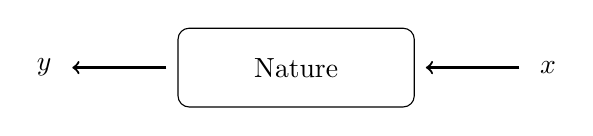
\begin{tikzpicture}[node distance=3.2cm, shorten >=4pt, ->]
        \tikzstyle{box} = [rectangle, rounded corners, minimum width=3cm, minimum height=1cm,text centered, draw=black, fill=white!100]
        \tikzstyle{arrow} = [thick, ->, shorten <= 4pt]
        
        \node (box) [box]{Nature};
        \node (y) [draw=none,fill=none, left of=box] {$y$};
        \node (x) [draw=none,fill=none, right of=box] {$x$};
        
        \draw [arrow] (x) -- (box);
        \draw [arrow] (box) -- (y);
    \end{tikzpicture}
\end{figure}
Inside the black box, nature associates the predictor variables with the response variables. We get to collect $y$ and $x$ as data, and the goal in analyzing them is twofold:
\begin{itemize}
    \setlength\itemsep{0cm}
    \item[] \textit{Understanding}. To extract some information about how nature is associating the response variables to the input variables
    \item[] \textit{Prediction}. To be able to predict what the responses are going to be when future inputs will be fed in
\end{itemize}
Similarly, there are two approaches towards these goals [\cite{Breiman2001}]:
\begin{itemize}
    \item \textit{The Data Modeling Culture}: The analysis starts by assuming a \textit{stochastic data model} for the inside of the black box, e.g. assuming that data are generated by independent draws from $y = f(x, \text{random noise}, \text{parameters})$, and then the values of the parameters are estimated from the data; model validation is performed based on goodness-of-fit tests and residuals analysis
    \item \textit{The Algorithmic Modeling Culture}: The analysis considers the inside of the box complex and unknown and the purpose is to find a function $f(x)$ -- an algorithm, a rule that operates on $x$ to predict the responses $y$; model validation is performed measuring predictive accuracy
\end{itemize}

These approaches differ in the logic used. The former start by trying to impose on nature a set of models -- often those the statisticians are comfortable with, well-known, whose properties are well studied -- and verifies that at least one of them is compatible with the data observed. The latter, on the contrary, is model-agnostic. Its ultimate target is finding \textit{a} rule that \textit{approximates} the mechanism associating inputs and outputs, even if this algorithm is convolute, inscrutable and unexpected, without imposing any a priori characteristics on the data-generating process. 

Breiman argues that statisticians in applied research consider data modeling as the main, if not the only, go-to for statistical analysis: 
\begin{displayquote}
    \say{I started reading the \textit{Annals of Statistics}, the flagship journal of theoretical statistics, and was bemused. Every article started with: \textit{Assume that the data are generated by the following model: ...}}
\end{displayquote}
The underlying assumption of the data modeling approach is that the parametric class of models imagined by the statistician for the complex mechanism devised by nature is indeed reasonable. Parameters are then estimated and conclusions are drawn. However, the conclusions drawn are about the model's mechanism, and not about nature's. Obviously, if the model is a poor approximation of nature, the conclusions may be wrong. On the other hand, a plus of data modeling is that it produces a simple and understandable description of the relationship between inputs and responses. This simplicity comes at the cost of uniqueness: different models, although equally valid, may give different descriptions of this relation. The fact that, following this approach, models are evaluated mainly using goodness-of-fit tests and other methods for checking fit, that yield a yes-no answer, creates difficulties in ranking the various models by quality [\cite{Breiman2001}]. The alternative proposed by the algorithmic culture is to measure the accuracy of the model's predictions: estimating the parameters in the model using the data and then using the model to predict the data checking how good the prediction is. The extent to which the model emulates nature's mechanics is a measure of how well the model can reproduce the natural phenomenon producing the data.

Sometimes approaching problems by looking for a data model imposes an a priori restriction to the ability of statisticians to deal with a wide range of statistical problems when they cannot be dealt with using models that remain enough understandable. The algorithmic community rarely make use of data models. Their approach starts by looking at the mechanics of how nature produces data as a black box partly unknowable. They stop at the mere acceptance of the fact that what is observed is a set of $x$'s that goes in and a set of $y$'s that comes out. The problem is rephrased as finding an algorithm, a rule $f(x)$, such that for future observed $x$, $f(x)$ will be a good predictor of $y$. The focus is shifted from data models to the properties of algorithms. The implicit assumption made in the theory is that the data is drawn $i.i.d.$ from an unknown multivariate distribution. The drawback of this approach is that models that best emulate nature in terms of predictive accuracy are also the most complex. 

Recent developments in both fields are trying to tie together these two cultures: this thesis goes in this direction, starting from the algorithmic approach and trying to extend it with concepts borrowed from the data modeling one. The philosophical underpinning throughout this work can be summarized as:
\begin{displayquote}
    The point of a model is to get useful information about the relation between the response and predictor variables. Interpretability is a way of getting information. But a model does not have to be simple to provide reliable information about the relation between predictor and response variables; neither does it have to be a data model. The goal is not interpretability, but accurate information [...] the emphasis needs to be on the problem and on the data -- \cite{Breiman2001}
\end{displayquote}
with a focus on the uncertainty regarding the information the model provides, i.e. its reliability in real life applications, that are the final purpose of all our efforts. Borrowing concepts from the Bayesian Nonparametric approach to statistics, we will try to construct the context around the algorithm. We will prove that any algorithm is a form of statistical modeling and that the separation from the two is not as clear-cut as Breiman suggests. That is why we will include algorithms into box of \textit{statistical modeling}.

How can we understand, concretely, the mechanics of nature? That depends on how nature manifests itself to us, namely what kind of data we are able to get. This shapes the way we can learn about nature from data and is the topic of the next section.




\section{Types of learning}\label{sec:types_of_learning}

All models, methods, techniques, algorithms, implemented to discover and understand the mechanics of nature are informally considered to perform a kind of leaning. This is true for any algorithm and, thus, also for neural networks. 

Therefore, neural networks can be viewed as a class of algorithms for statistical modeling and prediction. Based on a source of \textit{training data}, the aim is to produce a statistical model of the process, from which the data are generated: informally, we have to create a \say{story} for the data. Once we know the plot of the story, we can fill in the missing bits that the narrator has avoided telling us: what we call inference. We can distinguish three broad types of statistical modeling problems: \textit{density estimation}, \textit{classification} and \textit{regression}.

\textbf{Density estimation} problems are also referred to as \textbf{unsupervised learning} problems in the machine learning literature. In this class of problems, only the predictors are observed, no measurements of the outcome is provided. The learner's task is to describe how the data are organized or clustered, rather than make predictions [\cite{ESL}]. The goal is to model the unconditional distribution of data described by some vector $x$. 

\textbf{Classification} and \textbf{regression} problems are also referred to as \textit{supervised learning} problems in the machine learning literature. They only differ in the nature (discrete or continuous) of the target variable. In this class of problems we distinguish between \textit{input} variables, which we denote by $x$, and \textit{output} (or target) variables which we denote by the vector $y$. Classification problems require that each input vector $x$ be assigned to one of $K$ classes $\{y_1, \dots, y_K\}$ in which case the target variables represent class labels. Regression problems involve estimating the values of continuous variables $y$. Regression models and classification models both focus on the conditional density $p(y|x)$. Many regression techniques can be turned into classification methods by applying them to the problem of density estimation for the category probabilities. For example, if there are only two categories, we can denote them by $y \in \{0,1\}$. The regression problem is to model $E(y|x)$ that, thank to the definition of $y$, can be directly applied to the classification problem noting that $P(y = 1| x) = E[y|x]$. Hence, usually, any regression methods can be directly applied to classification [\cite{Lee2004}]. From the machine learning perspective, solving this class of problems entails learning an input-output mapping $f$ by examples: a function approximation task [\cite{ESL}]. This approximation, $f$, can be interpreted as, for example, $E(y|x)$.

Classification and regression problems can also be viewed as special cases of density estimation noting that the most general and complete description of the data is given by the probability distribution function $p(x,y)$ in the joint input-target space [\cite{Jordan1996}]. However, the usual goal is to be able to make good predictions for the target variables when presented with new values of the inputs. In this case it is convenient to decompose the joint distribution in the form:
$$p(x,y) = p(y|x) \; p(x)$$
and to consider only the conditional distribution $p(y|x)$. Seen in this form, it easy to assess how density estimation models can often arise more as components of the solution to a more general classification or regression problem -- since we may need an estimate of $p(x)$: to be able to estimate $p(x,y)$ or when there are missing data that we need to fill-in in a principled way. 

In what follows, we will focus on regression problems only: that is, the estimation of $p(y|x)$ from the data.





\section{The Anatomy of a Learner}
An informative high-level definition of learner, or learning algorithm, from a machine learning perspective is provided in \cite{Mitchell1997}:
\begin{displayquote}
    \say{A computer program is said to learn from experience \textit{E} with respect to some class of tasks \textit{T} and performance measure \textit{P}, if its performance at tasks in \textit{T}, as measured by \textit{P}, improves with experience \textit{E}}
\end{displayquote}
Of course, the variety of experiences, tasks, and performance measures is wide. Below a high-level overview of the possible instances of this concepts is provided:
\begin{itemize}
    \item Experiences \textit{E}: supervised or unsupervised learning
    \item Tasks \textit{T}: classification, classification with missing inputs, regression, anomaly detection, imputation of missing values, denoising, density estimation
    \item Performance measures \textit{P}: accuracy, error rate, goodness-of-fit tests
\end{itemize}
The starting point is the definition of a function approximator (or model). The statistician chooses an appropriate loss function according to the problem at hand. Once the loss function is chosen, an optimization criterion is defined, e.g. maximum likelihood, and an optimization routine must be set up. Typically the optimization problem is not solved analytically deriving a closed-form formula to provide a symbolic expression for the correct solution. On the contrary, updated estimates of the solutions are found via iterative processes\footnote{Optimization refers to the task of either minimizing or maximizing some function $J(\theta)$ by altering $\theta$. Since any maximization problem can be turned into a minimization problem, we will only consider minimization problems.}.

Therefore, all learning algorithms share a common \say{anatomy}:
\begin{enumerate}
    \item A specification of a dataset
    \item A model that defines a parametrised input-output mapping 
    \item A loss function that depends on the parameters of the model 
    \item An optimization procedure that finds the parameters values minimizing the loss function
\end{enumerate}
These components are modular: replacing them independently we can obtain a wide range of algorithms [\cite{Goodfellow-et-al-2016}]. The cost function typically includes at least one term that causes the learning process to perform statistical estimation. It may also include additional terms used for regularization.

This high-level description could be used for any algorithm as well as any statistical model! In the next section we will show that, in fact, they are two sides of the same coin. 





\section{Algorithms and Statistical models}
Given a dataset of pairs $\{y_i, x_i\}_{i=1}^{N}$, the simplest example of learning algorithm that can learn how to predict $y$ based on $x$ is linear regression. The underlying assumption is that the natural mechanics associating inputs and outputs can be described by a linear function mapping, $y = wx$. For each input-output pair, the model is a linear transformation of the inputs. Usually, a modified version of the model is used: an intercept term is added to the equation. This still preserves the linear mapping from parameters to predictions, but the mapping from features to predictions is now an affine function
$$y_i = w x_i + b$$
The intercept, in the machine learning literature, is often called the \textbf{bias}\footnote{This term is not related whatsoever to the idea of \textit{statistical bias}.} parameter (of the affine transformation) or \textbf{offset vector}. This nomenclature derives from the fact that, in the absence of any input, the transformation is biased towards $b$. 

Different parameters $w, b$ define different transformations. The goal is to find those values that minimize the errors in prediction, a procedure often referred to as \say{fitting} the model to data. There are many different methods to fit the model to data. To accomplish this task, the predictions are, thus, evaluated using a certain loss function. For continuous target variables the mean squared error (MSE) is often used: the values of $w$ and $b$ are chosen in a way that minimizes the residual sum of squares between the true outcomes and the predicted values.
$$\mathrm{MSE}(\theta) \stackrel{\scriptscriptstyle def}{=} J(\theta) = \sum_{i=1}^{N}\left\Vert y_i - (wx_i + b)\right\Vert_{2}^{2}, \quad \theta = (w,b)$$
where $\Vert\cdot\Vert$ is the $L^2$-norm (euclidean norm). The function $J$ will represent the \textit{loss} function henceforth, also called \textit{cost} or \textit{objective} function. Minimizing the loss function is the core of any machine learning algorithm. Therefore, there exists a tight relationship between learning and optimization. Optimizing a function requires being able to compute its derivative with respect to the parameters. 

Let's now build a story behind the algorithm. From a statistical point of view, we still assume that the true data-generating process can be described by a linear function mapping. However, in this case, we also assume that we are not able to observe the mechanics of nature directly: what we get to observe is a blurred picture of it. We call this \say{blurring} $\varepsilon$. We can, thus, rewrite the algorithm above as a statistical model where \say{statistical} comes from the fact that we are dealing with randomness. We collapse the intercept $b$ and $w$ into $\beta \stackrel{\scriptscriptstyle def}{=} (b, w)$, adding 1 as the first component of the vector of features, $x_i \stackrel{\scriptscriptstyle def}{=} (1, x_i)$. We make explicit an assumption often hidden when defining algorithms: our observations are independent and identically distributed. Thus we write
$$y_i = \beta x_i + \varepsilon_i \qquad \varepsilon \sim WN(0, \sigma^2)$$
where $WN$ stands for white noise. If we assume a specific parametric form for $WN$, e.g. a Gaussian distribution, we can write
$$y_i | x_i \stackrel{\scriptscriptstyle i.i.d.}{\sim} \mathcal{N}(\beta x_i, \sigma^2)$$
In this way we have defined a conditional probability $p(y|x)$. The toolbox of statistical inference contains various methods to estimate the parameter $\beta$ (and possibly $\sigma^2$). If, for example, we use the maximum likelihood approach, we would set the parameter to a value that maximizes the likelihood of our sample: again, we reduce inference (learning) to an optimization problem. In the Bayesian approach we would assign a prior to all uncertain quantities, in this case $\beta$, and use the Bayes' Theorem to compute the posterior of the parameters given the data.

We have now established a way to connect the two worlds and, strictly speaking, we have shown that what separates them is just the perspective from which we look at the problem. As soon as we assume that a certain degree of randomness exists, then we are in the realm of statistics. We thereby assert that for each algorithm there exists, perhaps not unique, a statistical interpretation.






\section{Neural Nets and Bayesian Nonparametrics}\label{sec:BNPreg}
Generally, the relation between $y$ and $x$ need not be linear. Indeed, in many interesting cases characterized by big and complex data (e.g. speech recognition, image processing) the mapping is better described by a nonlinear function. The regression model can be written in a general way as the combination of a deterministic regression function and a random residual
$$y = \underbrace{f(x)}_{\text{deterministic part}} + \underbrace{\varepsilon}_{\text{random part}}, \qquad \varepsilon \sim p_\varepsilon(\varepsilon)$$
As long as both, the regression function $f(\cdot)$ and the residual distribution $p(\cdot)$, are indexed by finitely many parameters, e.g. $(\beta, \sigma^2)$, inference reduces to a traditional parametric regression problem. The problem becomes a nonparametric regression when we wants to relax the parametric assumptions of either of the two model elements, that is the unknowns are not the parameters of a function, but the function itself.

Bayesian nonparametrics concerns Bayesian inference methods for \textit{nonparametric models}. A nonparametric model involves at least one infinite-dimensional parameter and hence may also be referred to as an \say{infinite-dimensional model}. Examples of infinite-dimensional parameters are functions or measures. The basic idea of nonparametric inference is to use data to infer an unknown quantity while making as few assumptions as possible. Usually, this means using statistical models that are infinite-dimensional. This characterization of nonparametric regression allows for three cases [\cite{MullerQuint2004}].

\paragraph{Nonparametric Residuals.} The model can be generalized by going nonparametric on the residual distribution, assuming $\varepsilon | G \stackrel{\scriptscriptstyle i.i.d.}{\sim} G$ with a nonparametric prior $p(G)$ on $G$, while keeping the regression mean function parametric as $f(\cdot) = f_\theta(\cdot)$  indexed by a (finite-dimensional) parameter vector $\theta$ with prior $p(\theta)$. We refer to this case as a \textit{nonparametric error model}. Essentially this becomes density estimation for the residual error. In principle, any model that is used for density estimation could be used. However, there is a minor complication. To maintain the interpretation of $\varepsilon$ as residuals and to avoid identifiability concerns, it is desirable to center the random $G$ at zero, for example, with $E(G) = 0$.

\paragraph{Nonparametric Mean Function.} One could, instead, relax the parametric assumption on the mean function and complete the model with a nonparametric prior $f(\cdot) \sim p(f)$. We refer to this as a \textit{nonparametric regression mean function}. Popular choices for $p(f)$ are Gaussian process priors [\cite{Rasmussen2006}] or priors based on basis expansions [\cite{Bishop2006}], regression trees [\cite{Breiman1984}], wavelet [\cite{vidakovic2009}], splines [\cite{Hastie1990, Denison}] or neural nets [\cite{Neal1996}]. Such methods can potentially approximate a wide range of regression functions. This approach, however, is  limited in the sense that it only allows for flexibility in the mean. Many datasets present non normality or multi-modality of the errors, degrees of skewness, or tail behavior in different regions of the covariate space. To capture such behaviors, a flexible approach for modeling the conditional density that allows both the mean and error distribution to evolve flexibly with the covariates is required.
    
\paragraph{Fully Nonparametric Regression.} One could go nonparametric on both assumptions. We refer to this as a \textit{fully nonparametric regression}. The sampling model becomes $p(y_i | x_i) = G_x$, with a prior on the family of \textit{conditional random probability measures}, $p(G_x, x \in \mathrm{X})$. Many commonly used priors for $\mathcal{G} = \{G_x\}$ are variations of dependent Dirichlet Process priors [\cite{Maceachern1999}].


\bigbreak

Although limited for the reasons we mentioned above, the \textit{nonparametric regression mean function} is a powerful tool, especially with the implementation of deep neural nets -- possible thanks to the advent of modern computers and the development of further numerical methods and software packages, e.g. \texttt{PyTorch} and \texttt{TensorFlow}. Usually, the residuals are assumed iid Gaussian with mean zero and with common variance. If this is the case, i.e. $\varepsilon$ has zero mean, then $f(x) = \mathrm{E}(y|x)$ becomes the \textit{conditional mean function}. When the assumption of a straight line (or a hyperplane) fit may be overly restrictive we may think to use a richer class of functions. The typical nonparametric regression model is of the form
$$y_i = f(x_i) + \varepsilon_i$$
where $f\in\mathcal{F}$, some class of regression functions. Nonparametric regression models differ in the class of functions to which $f$ is assumed to belong. The exist a variety of different ways to choose $\mathcal{F}$. There exist two classes that are very close to neural networks: local methods and basis functions.

\paragraph{Local methods.} These are some of the simplest approaches to nonparametric regression that operate locally. For example, in one dimension a moving average with a fixed window size would result in a step function. Sophistication can be added in the choice of the window, the weighting of the averaging, or the shape of the fit over the window. One example of such sophistication is \textit{kernel smoothing}: the idea is to use a moving weighted average, where the weight function is referred to as a kernel. A kernel is a continuous, bounded, symmetric function whose integral is one. Whatever the choice of the kernel, the resulting regression function estimate at a value $x$ of a single explanatory variable is 
$$\hat{y} = \frac{\sum_{i=1}^{n} y_i K(x-x_i)}{\sum_{i=1}^{n} K(x-x_i)}$$
The kernel regression approach is intertwined with work on kernel density estimation [\cite{Silverman1986, Loader2006}]. Kernels can be generalized to multiple dimensions, but data sparseness quickly becomes an issue. 

A completely different approach is to abandon the moving window in favour of partitioning the space into an exhaustive set of mutually exclusive regions. Using a constant function over the region gives rise to a step function. In one dimension, this is a histogram estimator [\cite{Gentle2002}, section 9.2]. In higher dimensions, a tree is a useful method for representing the splitting of the space into regions [\cite{Breiman1984}]. For regression, the predicted value is the average value of the response variable in a region, and for classification the fitted probability of class membership is the empirical probability in that region. 

\paragraph{Basis functions.} A large class of nonparametric methods are those that use an infinite set of basis functions to span the space of interest, e.g. $\mathcal{F}$ -- typically either the space of continuous functions or the space of square-integrable functions. The regression model becomes of the form
$$y_i = \sum_{k = 0}^{\infty} \beta_k \phi_k(x_i) + \varepsilon_i$$
where $\phi_1, \phi_2, \dots$ is a set of basis functions and, usually, $\phi_0$ is defined equal to 1 everywhere. 
An infinite number of terms would typically be required for a theoretical match to a continuous function, but in practice a finite number of terms is used to provide a close approximation to the infinite sum. We can obtain this imposing $k = 1,\dots,K$ and then to form a linear combination of these functions, so that for a sufficiently large value of $K$, and for a suitable choice of the $\phi_k(x)$, such a model has the desired \say{universal approximation} properties. Models of this form have the property that they
can be expressed as network diagrams in which there is a single layer of adaptive weights, also called \textbf{shallow learners} in the machine learning literature [\cite{Polson2017}].

An example of a basis set that spans the space of continuous functions is the standard basis of the vector space of all polynomials, $\{1, x, x^2, x^3, x^4, \dots\}$. Any continuous function can be approximated arbitrarily closely with a linear combination of these functions. Also mixture models can be basis representations, depending on the particular form of the model. One common form of a mixture model is the mixture of Gaussians: a collection of Gaussian densities is used as a basis set. For a univariate problem the model is
$$y_i = \sum_{k=0}^{\infty}\beta_k \phi\left(\frac{x_i - \mu_k}{\sigma_k}\right) + \varepsilon_i$$
where $\phi(u) = \frac{1}{\sqrt{2\pi}}\exp\{-u^2/2\}$ is the standard Gaussian density function, and $\mu_k$ and $\sigma_k$ are, respectively, the mean and standard deviation of the Gaussians in the mixture.


\section{Neural Networks}
We can now, naturally, introduce neural networks in the context of nonparametric regression. Neural networks are a particular case of basis function in which the basis functions are defined as $\phi_k^{w, b}(x) = \varphi(w_k x + b_k)$, where the scalar-valued nonlinear function, $\varphi$, is applied to the affine transformation of the inputs. The nonlinearity, also called \textbf{activation function}, is defined to be identical for all inputs. The most common activation function used are presented in figure \ref{fig:activation_functions}. The intermediate layer is called \textbf{hidden layer}. The dimesionality, $K$, of the hidden layer defines the \textbf{width} of the model, while the overall number of hidden layers determines the \textbf{depth} of the model -- being a plain neural network the depth is obviously one. 
\begin{figure}[ht]
    \centering
    \includegraphics[width=\textwidth]{images/activations.png}
    \caption{Most used activation functions.}
    \label{fig:activation_functions}
\end{figure}
Usually, layers are not interpreted as vector-to-vector functions. Rather, they are thought of as consisting of computational units or neurons, that act in parallel, each representing a vector-to-scalar function. This view highlights the inspiration of neural networks to the human brain. The univariate model can be written as
$$y_i = \sum_{k=0}^{K} \beta_k \; \phi_k^{w, b}(x) + \varepsilon_i$$
\begin{figure}
    \centering
    \includegraphics[scale=0.4]{images/nn.jpg}
    \caption{A stylized example of a fully-connected feedforward neural network. The input layer has four units, corresponding to the components of the vector $x_i \in \mathbb{R}^Q, \; i = 1,\dots, N$, with $Q = 4$. Each circle is a neuron calculates a weighted sum of an input vector plus bias and applies a nonlinear function to produce an output, which is this case is a scalar $y_i, \; i=1,\dots,N$, that is $D = 1$.}
    \label{fig:neural_network}
\end{figure}
This is the canonical example of neural network, known also as fully-connected feedforward neural network [\cite{Rosenblatt1958, Goodfellow-et-al-2016}]. Note that in the machine learning literature the basis functions are called \textit{hidden nodes}. For a historical review of neural networks and deep learning consult \cite{Schmidhuber2015}. 

It can be interpreted as a two-stage regression model: in the first stage the features are derived via a composition of an affine transformation of the inputs and a component-wise nonlinear function. These extracted features, in the second stage, are mapped to the output via a second affine transformation [\cite{ESL}]. In fact, also linear regression can be interpreted as a very simple example of neural network where $\varphi$ is an identity mapping. These models are associated with directed acyclic graphs, known as \textit{network diagram}. The neural network described above can be represented as in figure \ref{fig:neural_network}. To extend the above model to a multivariate $y$, we simply treat each dimension of $y$ as a separate output and add a set of connections from each hidden node to each of the dimensions of $y$. We can also assign an observation-specific residual variance.

It is clear from the equation above  that a (deep) neural network is simply a nonparametric regression using a basis representation. In other words, the key to understanding a neural network model is to think of it in terms of basis functions. 

From the equation above, it is also clear that a neural network is a standard parametric model, with a likelihood and parameters to be fit. We can, thus, claim that it is not a black box or purely an algorithm. It should now be apparent that neural nets are both algorithms \textit{and} statistical models. By viewing neural networks as statistical models, we can now apply many other ideas in statistics in order to understand, improve, and appropriately use these models. The disadvantage of viewing them as algorithms is that it can be difficult to apply knowledge from other algorithms. Taking the model-based perspective, we can be more systematic in discussing issues such as choosing a prior, building a model, checking assumptions for the validity of the model, and understanding uncertainty in our predictions [\cite{Lee2004, Polson2017}]. 

The neural network described above is an example of a shallow learner: informally, every model that cannot be categorized as deep is a shallow learner. Almost all shallow learners are data reduction techniques that consist of a low dimensional auxiliary variable $Z$ and a prediction rule specified by a composition of functions
$$f(x) = f_2\big(f_1(x)\big) = f_2(z), \qquad f_1(x) \coloneqq z$$
\begin{figure}[ht]
    \centering
    \includegraphics[scale=0.06]{images/nn_lr.png}
    \caption{The network graph of linear regression. For each observation, the predictor is a 3-D vector. The addition of the intercept has been made explicit.}
    \label{fig:lr_neural_network}
\end{figure}
Linear regression, Logistic regression, Principal component analysis, Partial least squares, Reduced rank regression, Linear discriminant analysis and Project pursuit regression are all examples of shallow learners. Furthermore, they all can be represented as a neural network, for example a linear regression network diagram is shown in figure \ref{fig:lr_neural_network}.



\section{Neural Nets as Graphical Models}
How can we represent conditional and unconditional distributions with neural networks? One way to answer this question is to find a suitable graph representation of probability distributions. Probabilistic Graphical Models (PGM) use diagrammatic representations to describe random variables and relationships among them. Similar to a graph that contains nodes (vertices) and links (edges), PGM has nodes to represent random variables and links to express probabilistic relationships among them. Below we will provide a simple example.

Consider a case in which we want to model the unconditional distribution $p(x)$. A general approach to density estimation is to treat the density as being composed of a set of $K$ simpler densities, where possibly $K=\infty$. This approach is a probabilistic form of clustering which involves modeling the observed data as a sample from a \textit{mixture density}:
$$p(x|\pi) = \sum_{i=1}^{K} \pi_i \; p(x|i, \theta_i)$$
where the $\pi_i$ are constants known as \textit{mixing proportions}, the $p(x|i, \theta_i)$ are the \textit{component densities}, generally taken to be from a simple parametric family, and $\theta_i$ are the parameters of the component densities. A common choice for component density is the multivariate Gaussian. In this case $\theta_i = (\mu_i, \Sigma_i)$. By varying this parameter, a wide variety of high-dimensional, multi-modal data can be modeled. Gaussian mixtures are representable as simple networks with one or more layers of adaptive weights, e.g. principal component analysis, canonical correlation analysis, kernel density estimation and factor analysis [\cite{Polson2017}], as shown in fig. \ref{fig:gaussianmix}. 
\begin{figure}
    \centering
    \includegraphics[scale=0.5]{images/gaussianmix.png}
    \caption{A network representation of a Gaussian mixture distribution. The input nodes representing the components of $x$ are in the lower level. Each link has a weight $\mu_{ij}$, which is the $j$-th component of the mean vector for the $i$-th Gaussian. Each node in the intermediate layer contains the covariance matrix $\Sigma_i$ and computes the Gaussian conditional probability $p(x|i,\mu_i,\Sigma_i)$. These probabilities are weighted by the mixing proportions $\pi_i$ in the last layer and the output node calculates the weighted sum $p(x) = \sum_i \pi_i p(x|i, w_i)$.}
    \label{fig:gaussianmix}
\end{figure}
Neural networks express relationships between variables by utilizing the representational language of graph theory. Variables are associated with nodes in a graph and transformations of variables are based on algorithms that \say{[...] propagate numerical messages along the links of the graph} [\cite{Jordan1996}]. The graphs is accompanied by probabilistic interpretations of the variables and their interrelationships. As we have seen, such probabilistic interpretations allow a neural network to be understood as a form of probabilistic model and reduce the problem of learning the weights of a network to a problem in statistics. Hidden Markov models and Dynamic Linear models -- also called Kalman filters in the machine learning literature -- are all examples of graphical probabilistic models. There is a strong relationship between these models and neural networks: it is often possible to reduce one kind of model to the other. Indeed, neural networks can be seen as members of a general family of probabilistic graphical models [\cite{Goodfellow-et-al-2016}, ch. 20].

Although elegant, this interpretation of the neural nets is limited since interpretability becomes easily an issue when the network grows deep. That is why it will not be treated in what follows. A more useful interpretation, is to look at neural nets as a highly nonlinear nonparametric function approximator, that is as a particular case of basis function.


\section{Deep Learners and Deep Neural Networks}
Deep learning refers to a wide class of machine learning techniques and architectures, with the common trait of \say{[...] using many layers of nonlinear information processing} [\cite{DengYu2014}]. In general, a deep learner, is a representation learning methods with multiple levels of representation, obtained by composing simple but nonlinear transformations of the raw data, with each of these transforming the representation at one level (starting with the raw input) into a representation at a higher level of abstraction. Composing enough of such transformations, very complex functions can be learned [\cite{LeCun2015}]. A deep architecture can be thought as a multilayer stack of simple models.

A \textbf{Deep Neural Net} (DNN) simply applies a composition of functions $\phi$, instead of a single one. Deep neural nets provide a flexible representations of $f(\cdot)$ capable of rendering nonlinear mappings which can approximate any given mapping to arbitrary accuracy. Given an input, $X \in \mathbb{R}^Q$, and an output, $Y \in \mathbb{R}^D$, usually both high-dimensional, the mapping $f: {R}^Q \rightarrow {R}^D$ is modeled via the superposition of univariate semi-affine functions where univariate activation functions are used to decompose the high-dimensional $X$, as a plain neural network. The particular characteristic of DNN is the depth of the networks, usually more than 2 hidden layers. Then a deep prediction rule can be expressed, in matrix notation, as:
\begin{align*}
    h^{(1)} &= \varphi_1 \left( W^{(0)}X + b_{0}\right)\\
    h^{(2)} &= \varphi_2 \left( W^{(1)}  h^{(1)} + b_{1}\right)\\
    &\cdots\\
    h^{(L)} &= \varphi_L \left( W^{(L-1)} h^{(L-1)} + b_{L-1}\right)\\
    f(X) &= W^{(L)} h^{(L)} + b_{L}
\end{align*}
where $h^{(l)}$ identifies the layer and the $\beta_k$'s have been collapsed in the matrix $W$, for each layer. DNN are, perhaps, the most famous inhabitant of this class of models in recent years, however other models characterized by deep architecture exists: deep gaussian processes [\cite{Damianou2013, Lee2017}] and neural processes [\cite{Garnelo2018a}] that are treated in the following chapters.

How a series of simple operation can represent complicated mappings? In other words, why this approach works? The formal roots of DL can be traced back in Kolmogorov's representation of a multivariate response surface as a superposition of univariate activation functions applied to an affine transformation of the input variables [\cite{Kolmogorov1957}]. In 1957 the Russian mathematician Kolmogorov showed that \textit{any} continuous function $f$ of many variables can be represented as a composition of addition and
some functions of one variable. The original version of this theorem can be expressed as follows\footnote{We propose a version of the theorem deducted from \cite{Kolmogorov2009, Kolmogorov2011}.}:
\begin{theorem}[Kolmogorov–Arnold superposition theorem]
    Let $f: [0, 1]^{d} \rightarrow \mathbb{R}$ be an arbitrary multivariate continuous function defined on the identity hypercube. Then it
has the representation 
$$f(\mathbf{x}) = f(x_1, \dots, x_d) = \sum_{q=0}^{2d} \phi_q \left(\sum_{p=1}^{d} \psi_{q,p} (x_p) \right)$$
with continuous one–dimensional inner and outer functions $\phi_q$ and $\psi_{q,p}$, defined on the real line. The inner functions $\psi_{q,p}$ are independent of the function $f$.
\end{theorem}
Starting from the 2000s, Kolmogorov’s superposition theorem found the attention of the machine learning community interest in providing a theoretical justification of neural networks. Hecht–Nielsen’s [\cite{Kolmogorov2011}] tries to apply the theorem to a feed-forward network with an input layer, one hidden layer and an output layer [\cite{Kolmogorov1987}]. However, the inner functions, $\psi$, in this application of the theorem are highly nonsmooth and thus not useful in optimization. Sprecher [\cite{Kolmogorov1965}] contributed to this research topic providing an explicit method to construct the univariate functions $\psi$, corresponding to the activation functions of the network. Bryant [\cite{Bryant2008}] implements Sprecher's [\cite{Kolmogorov1972}] algorithm to estimate the inner link function. In his application of the theorem, deep layers allow for smooth activation functions to provide \say{learned} hyperplanes which find the underlying complex interactions and regions without having to see an exponentially large number of training samples.

To summarize, deep learning architectures rather than manually engineering the transformations to be applied to create more abstract concepts, learn them: the behaviour of the hidden layers is not directly specified in the data, it is learned. 












%start numbering
%Ornament at the end of chapter
\begin{center}
   \pgfornament[width=6cm, scale=1]{89} 
\end{center}




%------------------------- Chapter 2 -------------------------
\chapter{The Learning Process}

%epigraph
% \renewcommand{\epigraphsize}{\small}
% \setlength{\epigraphwidth}{0.5\textwidth}
% \setlength{\epigraphrule}{0mm}
% \renewcommand{\textflush}{flushright}
% \epigraph{\itshape\say{Recall seeing a package to make quotes}}{\scshape Snowball}

The goal of the learning process of any learning algorithm is to minimize the expected generalization error, known as \textbf{risk}, i.e. to maximize its accuracy when new inputs are provided. This is achieved via two paths: \textbf{optimization}, which is the process of finding parameters values that minimize the loss function, and \textbf{regularization} which is the process of reducing model capacity avoiding overfitting on the observed data, the \textbf{training set}, and improve generalization performances. To use Mitchell's codification [\cite{Mitchell1997}], we care about some performance measure $P$, that is defined with respect to new unseen observations, the \textbf{test set}.

To measure the generalization performance of the model we compute the loss function, e.g. the MSE, of the model on the new, unseen data. For this purpose, often in practical applications the dataset is divided into training set, used to perform the learning process, and test set, used to measure out-of-sample performances. Sometimes, especially for DL, a third partition is created called \textbf{validation set} and is used to learn the hyperparameters of the model, if not calibrated ex-ante. If not explicitly declared, $N$ will refer to the number of observations in the training set and $N^{test}$ and $N^{val}$ will refer, respectively, to the test and validation set.

To improve generalization performances means to reduce the loss on the test set, $J_{test}$. However, only the training data are used to train the model. One can intuitively minimize the loss, $J_{train}$ on the training set, simply solving for where its gradient is $\nabla_{\theta}J_{train} = 0$, and hope this will lead to improvements on the test set. What we actually care about is the generalization error, computed on the unobserved data. How can we affect the performance on the test set when we can observe only the training set? Statistical theory comes handy in justifying this. We are able to do so thanks to the implicit assumption (\cref{sec:cultures}) that the training and test set are produced by the same data-generating process and each observation is independent of any other. 

Now that we have justified why it is sensible to minimize the loss function on the observed data, how do we actually minimize it? In other words, how do we choose the value for the parameter $\theta$ which minimizes our loss function producing \say{good} estimates $\hat{y}(x)$? 

In the machine learning literature, learning or inference is always cast as an optimization problem. In the next section we will give an overview of the procedures.



\section{Optimization}\label{sec:optimization}
The aim of optimization is to find values of parameter $\theta$ in the parameter space $\Theta$ that minimize the loss function $J(\theta)$, which usually includes a term specifying a performance measure evaluated on the training set and a regularization term to improve the generalization error and avoid overfitting which will be discussed in the next section.

Note that for the purpose of this thesis, we will treat optimization in a supervised learning context, i.e. we are provided with the outcome variable $Y$ as well as the inputs $X$. Furthermore, throughout this section, we will refer to the unregularized optimization case, i.e. the loss function will not contain any regularization term. The development of the regularized cases will be addressed in the next section.

It is common in machine learning applications to use loss functions that decompose as a sum over some per-example loss functions. Therefore, up to a multiplicative constant, the cost function can be seen as an expectation [\cite{Goodfellow-et-al-2016}]. In principle, we would like to minimize the objective function where the expectation is taken over the data-generating distribution, $p_{data}$:
\begin{equation}
    J^\star(\theta) = \mathrm{E}_{(X, Y) \sim p_{data}} L\left( f_\theta(x), y \right) \label{risk}
\end{equation}
that defines the risk, i.e. the expected generalization error, while $f_\theta(x)$ defines the predicted output when the input is $x$.

However, in practise we only have a finite training set. Therefore, we are bound to use a reduced form of $J^\star(\theta)$, namely the \textbf{empirical risk} defined as
\begin{equation}
    J(\theta) = \mathrm{E}_{(X, Y) \sim \hat{p}_{data}} L\left( f_\theta(x), y \right) = \frac{1}{N} \sum_{i=1}^{N} L\left( f_\theta(x_i) ; y_i \right) \label{empirical_risk}
\end{equation}
where $\hat{p}_{data}$ is the empirical distribution on the training set. Therefore, rather than optimizing the risk directly, the empirical risk is minimized with the hope that the risk decreases as well -- a procedure called empirical risk minimization. 

The most important mathematical tool used for optimization is the derivative operator, denoted as $J'(\theta)$ or $dJ/d\theta$. The concept of derivative is crucial for optimization algorithms because it specifies how to scale a small change in the parameters $\theta$ to obtain the corresponding change in the loss function valuation 
$$J(\theta + \eta) \approx J(\theta) + \eta J'(\theta)$$
It tells us that $J(\theta)$ can be reduced by moving $\theta$ in small steps with the opposite sign of the derivative. The type of optimization techniques employing the derivative concept as tool is called \textbf{gradient-based} optimization. In machine learning this is the most used class of methods and will be the object of this section.

How does gradient-based optimization work? Since, as said, often loss functions decompose as a sum over some per-example loss function, the computation of the gradient is performed using the linearity of the derivative operator
\begin{align}\label{gradient}
    g = \nabla_{\theta} J(\theta) & = \nabla_{\theta} \mathrm{E}_{(X, Y) \sim \hat{p}_{data}} L\left( f_\theta(x) ; y \right)\\ \nonumber
    & = \nabla_{\theta} \frac{1}{N} \sum_{i=1}^{N} L\left( f_\theta(x_i) ; y_i \right) \\ \nonumber
    & = \frac{1}{N} \sum_{i=1}^{N} \nabla_{\theta} L\left( f_\theta(x_i) ; y_i \right)  
\end{align}
The most basic example of gradient-based optimization algorithm is \textbf{gradient descent} [\cite{Cauchy1847, Bishop2006}]. It proposes a new parameter value according to the updating rule
\begin{equation}
    \theta^{new} \leftarrow \theta - \lambda g \label{update_rule}
\end{equation}
where $\lambda \in \mathbb{R}$ is an hyperparameter called the \textbf{learning rate}, a positive scalar determining how the gradient affects the proposed value\footnote{Its determination has posed serious challenges to both practitioners and researchers. In subsection (\cref{sec:learning_rate}) we will review ways to set the parameter. Usually for \say{vanilla} gradient descent it is kept fixed during the entire optimization.}.

One issue in applying gradient descent is that, when the data is big, computing the expectation in eq. \eqref{gradient} is computationally very expensive since before an update is proposed, the model must be evaluated on the entire dataset in order to compute the per-example loss. Optimization methods that use the entire training set to compute the gradient are called \textbf{batch} gradient methods. One way to solve the issue is to resort to statistical estimation. Instead of computing the exact gradient, it is approximated by randomly sampling a small number of examples from the training set, computing the per-example loss, and taking the average over them only. This type of optimization methods is called \textbf{minibatch} or \textbf{stochastic} methods. Of course, to compute an unbiased estimate of the expected gradient, minibatches must be selected truly randomly. It can be shown\footnote{\cite{Goodfellow-et-al-2016} pp. 273-274.} that when the stochastic gradient is computed on different observations -- i.e. no observation is resampled -- the approximate expected gradient follows the gradient of the true generalization error, eq. \eqref{risk}. Each time the training set is fully sampled, the procedure restarts again. Each of this iterations is usually called \textbf{epoch}.

The basic example of a stochastic optimization method is \textbf{stochastic gradient descent}. The update rule for the parameters is the same as in eq. \eqref{update_rule} but instead of an exact $g$, an approximate $\hat{g}$ is used. The learning rate usually is not held fixed, but it is gradually decreased over time. This is necessary since the estimation of $g$ introduces noise, via the random sampling, that does not vanish even when a minimum is reached. Adaptive learning rate methods are discussed below. On the contrary, batch optimization methods, such as gradient descent, can hold $\lambda$ fixed over time\footnote{For more details on how to tackle the issue, the reader is redirected to \cite{Goodfellow-et-al-2016} ch. 8.},

Another example of stochastic optimization is the \textbf{momentum} method. This algorithm adds a variable $v$, called \textit{velocity}, that stores value of an exponentially decaying moving average of the past gradient and suggests the algorithm to move in the same direction. A memory parameter $\alpha \in [0,1)$ determines how much past information to store. The update rule becomes, denoting the size of the minibatch with $m$, 
\begin{align*}
    v^{new} & \leftarrow \alpha v - \lambda \nabla_{\theta} \left(\frac{1}{m} \sum_{i=1}^{m} L\left( f_\theta(x_i) ; y_i \right)\right), \quad m < N\\
    \theta^{new} & \leftarrow \theta + v^{new}
\end{align*}
Given $\lambda$ -- that should be modeled to vary in some ways -- the size of the step now depends on how large and aligned the sequence of gradients is.

A slightly modified version of the momentum algorithm is the \textbf{Nesterov momentum}. The gradient is evaluated after the velocity is applied. The update rule in this case is
\begin{align*}
    v^{new} & \leftarrow \alpha v - \lambda \nabla_{\theta} \left(\frac{1}{m} \sum_{i=1}^{m} L\left( f_{\theta+\alpha v}(x_i) ; y_i \right)\right)\\
    \theta^{new} & \leftarrow \theta + v^{new}
\end{align*}

It is important to note that given the common non-convexity of loss functions in deep learning, an important factor impacting the convergence of optimization algorithms is parameter initialization, i.e. the starting point of the path towards the minimum. This is the reason why, sometimes optimization is brought about using a completely different approach: training a simpler model and use the trained parameters as initial values of the more complex model. This technique is called \textit{supervised pretraining} [\cite{Goodfellow-et-al-2016}]. 




\subsection{The learning rate problem} \label{sec:learning_rate}
The convergence speed of SGD depends on the variance of the gradient estimates which, in turn, depends on the size of the mini-batch: by the law of large numbers, increasing the mini-batch size reduces the stochastic gradient noise. Smaller gradient noise allows for larger learning rates and leads to faster convergence. For \say{vanilla} gradient descent where we use the entire dataset, the learning rate can be relatively bigger with respect to using stochastic gradient descent.  Therefore, there is a trade-off between the computational overhead associated with processing a mini-batch of a bigger size, and the computational cost of performing more gradient steps due to the smaller learning rate. 

To accelerate the learning procedure, one can either optimally adapt the mini-batch size for a given learning rate, or optimally adjust the learning rate to a fixed mini-batch size. The latter approach is the preferred in the machine learning literature. 

How does the learning parameter need to be chosen? This question has multiple answers, each corresponding to a different algorithm. Here we briefly review the most important that will be useful in actual applications. The basic idea is that in each iteration, the empirical gradient variance can guide the adaptation of the learning rate which is inversely proportional to the gradient noise. Popular optimization methods that make use of this idea include

\paragraph{Delta-bar-delta.} The delta-bar-delta [\cite{Jacobs1988}] algorithm was one of the first heuristic method to adapt the learning rate of batch optimization methods. The rule is simple: if the partial derivative of the loss with respect to a given model parameter remains the same sign, then the learning rate should increase, otherwise the learning rate should decrease. 

\paragraph{AdaGrad.} A similar heuristic approach is AdaGrad [\cite{Duchi2011}] that scales the individual model parameters inversely proportional to the square root of the sum of all the historical squared values of the gradient. 

\paragraph{RMSProp.} A modification of AdaGrad is provided by the RMSProp algorithm [\cite{Hinton2012}]. It changes the gradient accumulation into an exponentially weighted moving average commanded by an hyperparameter $\rho$ determining the algorithm's memory. 

\paragraph{Adam.} The Adam algorithm combines RMSProp to learn the learning rate with the momentum method [\cite{Adam2014}].


\section{Regularization} 
As said, the aim of a learning algorithm is twofold: minimizing the training error and the the gap between training and test error. In other words, avoiding
\begin{itemize}
    \item \textbf{Underfitting}: high error rate on the training set
    \item \textbf{Overfitting}: large gap between training error and generalization error
\end{itemize}
We can control whether a model is more likely to overfit or underfit by altering its \textbf{capacity}, that is its ability to fit certain variety of functions -- e.g. linear regression as a lower capacity than polynomial regression -- and one way to control the capacity of a learning algorithm is by choosing its \textbf{hypothesis space}, the set of functions that the learning algorithms is able to approximate, appropriately.

Regularization refers to strategies designed to reduce the generalization error, often paying the price of higher training error. They can all be seen as a way to reduce the capacity of the model. In general such strategies can be categorized into two classes: 
\begin{enumerate}
    \item Strategies that put extra constraints on a learning model  (e.g. adding restrictions on parameters' values or on the activation functions)
    \item Strategies that add extra terms in the objective function
\end{enumerate}
These constraints and penalties can be generally interpreted as encoding some specific kind of prior knowledge or expressing preferences for simpler model classes in order to improve generalization reducing the threat of overfitting.

In the context of deep learning, most regularization strategies are based on regularizing estimators that have the effect of increasing bias while reducing variance. As usual, the bias of an estimator is defined as $\text{Bias}(\hat{\theta}) = \mathrm{E}_{\hat{p}_{data}}(\hat{\theta} - \theta)$ which defines the expected error of the estimator, while the variance $\mathrm{V}(\hat{\theta})$ defines the error in the estimation stemming from the sensitivity to small fluctuations in the sample observed. High bias can cause an algorithm to mistake the mapping between features and target outputs (underfitting), while high variance can cause an algorithm to model the random noise in the training data rather than the intended outputs (overfitting). Therefore, an effective regularizer is one that is able to find the right trade-off, reducing variance significantly while not overly increasing the bias. 

Via regularization we want to restrict at minimum the capacity of the model to include the data-generating process ruling out other possible candidate data-generating processes in the scope of the model capacity (reducing the variance). This conditions of the model capacity should not be too restrictive: the risk is to rule out of the scope of the model capacity the true data-generating process (bias). Unfortunately, we almost never have access to the true data-generating process and thus we can never be completely sure that the class of models estimated includes the true generating process. 




\subsection{Parameter Norm Penalties} \label{subsec:parameter_norm}
A commonly used example of regularization approach belonging to the second class of strategies are the \textbf{parameter norm penalties}. These approach entails limiting the capacity of the model by adding a penalty in the loss function $J(\theta)$ proportional to the \textit{parameter norm} $\Omega(\theta)$. Note that usually for neural networks the norm is computed only on the weights $W$, while the biases $b$ are left unregularized. The regularized cost function can be written as
\begin{equation}
    \tilde{J}(\theta) = J(\theta) + \alpha \Omega(\theta)
\end{equation}
where $\alpha \in [0, \infty)$ weights how the norm penalty affects the regularized objective function relative to the standard loss function. In neural networks, usually, the penalties are separated per layer and a different $\alpha$ is used for each layer. In practical applications, due to computational costs, the definition of $\Omega$ used is often the same for each layer. Different definitions of $\Omega$ result in different solutions being preferred. The two widely known definitions used are:

\paragraph{$L^2$-norm.} In this case we have $\Omega(\theta) = \frac{1}{2}\Vert \theta \Vert_{2}^{2}$, commonly known as \textbf{weight decay}. Therefore the regularized loss becomes
\begin{align*}
    \tilde{J}(\theta) &= \frac{\alpha}{2} \theta^\top \theta + J(\theta)\\
    \nabla_{\theta} \tilde{J}(\theta) &= \alpha \theta + \nabla_{\theta} J(\theta)\\
    \intertext{defining the update rule}
    \theta^{new} &\leftarrow \theta - \lambda \big( \alpha\theta + \nabla_{\theta}J(\theta) \big)
\end{align*}
The effect of the regularization term is to shrink $\theta$ by a constant factor on each step, just before performing the usual gradient update.

\paragraph{$L^1$-norm.} In this case we have $\Omega(\theta) = \Vert \theta \Vert_{1} = \sum_{i}|\theta_i|$, obtaining
\begin{align*}
    \tilde{J}(\theta) &= \alpha \Vert \theta \Vert_{1} + J(\theta)\\
    \nabla_{\theta} \tilde{J}(\theta) &= \alpha sign(\theta) + \nabla_{\theta} J(\theta)
\end{align*}
In this case, the gradient does not scale linearly as with the $L^2$-norm definition, but it is a constant factor with a sign equal to the sign of $\theta$. The gradient so defined has no longer an algebraic solution and must be approximated. It can be shown [\cite{Goodfellow-et-al-2016}] that $L^1$ regularization results in a solution that is more sparse, i.e. parameters will tend to have optimal value of zero. This can be interpreted as a form of variable selection mechanism. The LASSO is an example of this mechanism employed in linear models training. 

The parameter norm penalties regularization can also be interpreted as MAP Bayesian inference: e.g. $L^2$ regularization is equivalent to MAP Bayesian inference with a Gaussian prior on $\theta$.




\subsection{Early Stopping}\label{subsec:early_stopping}
Often when training neural network with sufficient representational capacity, a signal that the model is overfitting is that training error decreases steadily over time, but validation set error begins to rise again. The validation set is used to evaluate a given model, like the test set, frequently during training. It corresponds to a small portion of the data that are mainly used to fine-tune the model hyperparameters. Hence the model \say{occasionally} sees the validation data, but never learns from them.

In principle, we can expect that minimizing the validation set error would also lead to better test error. Therefore, rather than stopping the optimization algorithm when the training error is minimum, it is possible to stop it earlier, when the validation error is the least, i.e. we use the parameters values in correspondence of the least validation error, rather than the latest values returned by the optimization algorithm. 

This strategy is known as early stopping. In practise, the optimization algorithm is instructed to stop when no parameters have improved over the best recorded validation error for some pre-specified number of iterations. In deep learning, this is the most commonly used regularization strategy. In this way, we control how many times the optimization algorithm can run to fit the training set, limiting the threat of overfitting. This strategy does not require any change in the underlying procedure, loss function, or parameter set.



\subsection{Sparse Representations}
Another approach to regularize neural networks is to impose a penalty on the activation functions of the units by introducing sparseness. Essentially, the model is brought to prefer configurations in which more hidden units are set to zero; this reduces the capacity of the model. Indirectly, it is like imposing a complex penalization on the model parameters, As mentioned in subsection (\cref{subsec:parameter_norm}), also $L^1$-penalization introduces sparseness in the parameters values. 

Sparseness is induced in the representations, i.e. components of the hidden layer $h_l$ are set to zero, not in the components of the parameters $W_l$ or $b_l$. In practice, this regularization is applied to the model via adding a parameter norm penalty over the dimension of the hidden units in the loss function
\begin{equation*}
    \tilde{J}(\theta) = J(\theta) + \alpha \Omega(h), \quad \alpha \in [0,\infty)
\end{equation*}
Note how the argument of $\Omega$ is now the $h$ vector and not $\theta$.



\subsection{Bagging and Ensemble Methods}\label{subsec:bagging}
The underlying idea is to reduce generalization error combining different models. In practise it is performed by training different models separately and for each input, $X_i$, each of these models collect the proposal $f_i(X_i)$. Techniques using this strategy, known as \textit{model averaging}, go under the label of \textbf{ensemble methods}.

On average the ensemble performs at least as well as any of its members. In case the errors made by the individual models are independent, the ensemble performs significantly better than them.

A particular example is the \textbf{bagging} method, short for \say{bootstrap aggregating}. This approach allows the very same model to be reused, instead of fitting different models. In practise $k$ dataset with the same number of observations of the training set are constructed by sampling with replacement from the training set. Model $i$ is trained on dataset $i \in \{1, \dots, k\}$. Given that the same model is used, the difference among the models in the ensemble is due to the different $k$ \say{artificial} dataset on which the model is trained.



\subsection{Dropout}
\textbf{Dropout} is a type of ensemble method, but for the importance it will have in this thesis -- and in practise -- it deserves a dedicated subsection. 

Bagging entails training the same model multiple times on different training sets. For large neural networks the computational cost soon skyrockets. Dropout provides a computationally inexpensive approximation to train and evaluate a \textit{bagged} ensemble. In particular, dropout trains the ensemble consisting of all subnetworks that can be formed by removing non-output units from the underlying base network. The number of submodels, thus, grows exponentially in the number of units. Switching off a unit -- in the input layer or hidden layers -- is performed by multiplying it by zero. Dropout applied to input units serves as a form of variable selection [\cite{Hinton2006, Srivastava2014}], interpretable as Bayesian ridge regression [\cite{Polson2017}]. When applied to hidden layers it regularizes the choice of the number of hidden units in a layer. Once a variable from a layer is dropped, all terms above it in the network also disappear.

In practise, dropout removes units in the input layer and/or in the hidden layers randomly with a given
probability $p$, different for each layer. Training with dropout is performed using stochastic optimization methods like SGD. Each time a minibatch is created, for each layer, a binary vector $\zeta_l$ is randomly sampled, where each component is distributed as a $\mathrm{Bernoulli}(p_l)$. The number of components in the binary vector matches the number of units in the layer. This vector is usually called \textbf{mask}. The components of $\zeta$ are sampled independently of each other. The probabilities $p_l$ are hyperparameters fixed before training begins. Therefore the original input layer becomes $\tilde{x} = x \odot \zeta_0$, where $\odot$ represents the Hadamard (or element-wise) product. Similarly, each hidden layer becomes $\tilde{h}_l = \zeta_l \odot h_l, \; l = 1, \dots, L$. The same values of the binary vector are used during optimization, namely when performing back-propagation. 

Let $J(\theta, \zeta)$ define the cost of the model defined by parameters $\theta$ and the mask $\zeta$.
Marginalizing over the randomness, the objective becomes 
$$\mathrm{E}_{\zeta \sim \mathrm{Ber}(p)} J(\theta, \zeta)$$
The expectation contains exponentially many terms, but an unbiased estimate of its gradient can be obtained by sampling and using only certain values of $\{\zeta_0, \dots, \zeta_L\}$. This differentiate dropout from bagging: in the latter case, each model is trained until convergence on its respective training set; in the former case, most models are not explicitly trained at all, but only a tiny fraction of the possible subnetworks are trained for a single step, and the parameter sharing, across models with the same active units, causes the remaining subnetworks to arrive at good settings of the parameters. 

To conclude, we have to highlight that optimization, per se, does not provide an uncertainty measure. This is solve by taking a Bayesian approach.







\section{Bayesian Neural Networks}
Bayesian Neural Networks (BNN) were first suggested in the '90s and studied extensively since then [\cite{MacKay1992, Neal1996}], they are now living a period of huge fame. They offer a probabilistic interpretation of neural networks models by inferring distributions over the models' weights (usually biases are left unbounded). The model offers robustness to overfitting, uncertainty estimates, and can easily learn from small datasets. As in any Bayesian inference problem, BNN place a prior distribution over a neural network’s weights, which induces a distribution over a parametric set of functions. 

Given training inputs $x$ and their corresponding outputs $y$, in Bayesian (parametric) regression we would like to find the parameters $\theta$ of the function $f_\theta$ such that $y = f_\theta(x)$, i.e. those values of the parameters that are likely to have generated the outputs. Following the Bayesian approach we would put some prior distribution over the space of parameters, $p(\theta)$. This distribution represents our prior belief as to which parameters are likely to have generated our data before we observe any data points. Once some data are observed, this distribution will be transformed to capture the more likely and less likely parameters given the observed data points. To perform inference, we further need to define a likelihood distribution, i.e. the model for our data, $p(y|x, \theta)$ -- the probabilistic model by which the inputs generate the outputs given some parameter setting $\theta$. 

We then look for the posterior distribution over the space of parameters by invoking the Bayes' theorem:
\begin{equation}
    p(\theta|x,y) = \frac{p(y|x, \theta) \; p(\theta)}{p(x)} \label{eq:posterior}
\end{equation}
where $p(x) = \int p(y|x, \theta) p(\theta)\; d\theta$. Once we compute this posterior, we can predict an output for a new input point $x^*$ by integrating out the parameters
$$p(y^*|x^*) = \int p(y^*|x^*, \theta) \; p(\theta|x,y) \; d\theta$$
Performing this integration is also referred to as \textit{marginalising} the likelihood over $\theta$, which explains the alternative name for the model evidence: \textit{marginal likelihood}. Marginalisation can be done analytically for simple models such as Bayesian linear regression. In such models the prior is conjugate to the likelihood, and the integral can be solved with known tools of calculus. Marginalisation is the one of core parts in Bayesian modelling, and ideally we would want to marginalise over all uncertain quantities -- i.e. averaging with respect to all possible model parameter values $\theta$, each weighted by its plausibility $p(\theta)$. But with more interesting models (even basis function regression when the basis functions are not fixed) this marginalisation cannot be done analytically. In such cases an approximation is needed.




\section{Variational Inference}\label{sec:VI}
Modern research in BNN often relies on either \textit{variational inference}, or \textit{sampling based techniques} like MCMC. Each approach has its merits and its limitations. MCMC methods tend to be more computationally intensive than variational inference but they also provide guarantees of producing (asymptotically) exact samples from the target density [\cite{RobertCasella2005}]. Variational inference does not enjoy such guarantees -- it can only find a density close to the target -- but tends to be faster than MCMC. Because it rests on optimization, variational inference easily takes advantage of methods like stochastic optimization and distributed optimization. Also some MCMC methods can also exploit these innovations [\cite{Welling2011}], but they are still not well established as variational inference. 

To provide an overview of the method, let's setup the general problem. Consider a joint density of latent variables $z = (z_1,\dots,z_m)$ and observations $x = (x_1,\dots, x_n)$. For example, in the case of a Gaussian distribution with unknown mean and variance, $z = (\mu, \sigma^2)$. In the case of a neural network, $z$ is equal to all weights in the network. We can write 
$$p(x,z) = p(z)\;p(x|z)$$
A typical Bayesian model draws the latent variables from a prior density $p(z)$ and then relates them to the observations through the likelihood $p(x|z)$. Inference, thus, amounts to conditioning on data and computing the posterior $p(z | x)$. In complex Bayesian models, like neural nets, this computation often requires approximate inference. 

As discussed above, the dominant paradigm for approximate inference has been MCMC. In MCMC, we first construct an ergodic Markov chain on $z$
whose stationary distribution is the posterior $p(z|x)$. Then, we sample from the chain to collect samples from the stationary distribution. Finally, we approximate the posterior with an empirical estimate constructed from a subset of the collected samples. 

The key characteristic of variational inference is that it transforms inference problems into optimization. Thus, variational inference is suited to large data sets and scenarios where we want to quickly explore many models; MCMC is suited to smaller data sets and scenarios where we are willing to pay a heavier computational cost for more precise samples. 



\subsection{Preliminaries}
First, we assume a family of approximate densities $\mathcal{Q}$, that is a set of densities over the space of the latent variables. Then, we try to find the member of that family that minimizes the Kullback-Leibler
(KL) [\cite{KL1951}] divergence from the exact posterior,
\begin{equation}
    q^\star(z) = \underset{q(z)\in\mathcal{Q}}{\arg \min} \; \mathrm{KL}[q(z)\Vert p(z|x)] 
    \label{eq:VI}
\end{equation}
Finally, we approximate the posterior with the optimized member of the family $q^*(z)$. In other words, the goal in VI is to approximate the posterior by a simpler distribution. To this end, one minimizes the KL  divergence between the approximating distribution and the posterior. One of the key ideas behind variational inference is to choose $\mathcal{Q}$ to be flexible enough to capture a density close to $p(z | x)$, but simple enough for efficient optimization.

Unfortunately, the objective, \eqref{eq:VI}, is not computable because it requires computing the evidence $\log p(x)$. In fact $p(z|x) = p(x,z)/p(x)$. To appreciate this recall that the KL divergence is
\begin{align}
    \mathrm{KL}[q(z)\Vert p(z|x)] &= \mathrm{E}[\log q(z)] - \mathrm{E}[\log p(z|x)] \nonumber\\
    \intertext{where all expectations are taken with respect to $q(z)$. Expanding the conditional,}
     &= \mathrm{E}[\log q(z)] - \mathrm{E}[\log p(z, x)] + \log p(x) \label{eq:KL}
\end{align}
and the dependence on the log-evidence is revealed.

Since we cannot compute the KL, we optimize an alternative objective that is equivalent to the KL up to an \textit{added} constant,
$$\mathrm{ELBO}(q) = \mathrm{E}[\log p(z, x)] - \mathrm{E}[\log q(z)]$$
This function is called the \textbf{evidence lower bound} (ELBO). The ELBO is the negative KL divergence in eq. \eqref{eq:KL} plus $\log p(x)$, which is a constant with respect to $q(z)$. Maximizing the ELBO is equivalent to minimizing the KL divergence in eq. \eqref{eq:KL}. To make explicit the dependence of the ELBO on the conditional log-likelihood of the data given the latents, we can rewrite $p(z,x) = p(x|z)p(z)$, thus
\begin{align}
    \mathrm{ELBO}(q) &= \mathrm{E}[\log p(x|z)] + \mathrm{E}[\log p(z)] - \mathrm{E}[\log q(z)] \nonumber\\
                &= \mathrm{E}[\log p(x|z)] - \mathrm{KL} [q(z)\Vert p(z)] \label{eq:ELBO}
\end{align}
The first term is the expected likelihood: it encourages densities that place their mass on configurations of the latent variables that explain the observed data. The second term is the negative divergence between the variational density and the prior: it encourages densities close to the prior. Thus the variational objective mirrors the usual balance between likelihood and prior. The KL term can also be interpreted as a form of regularization that favours simpler models. 

Furthermore, rewriting eq. \eqref{eq:KL} as 
$$\log p(x) = \mathrm{KL} [q(z)\Vert p(z | x)] + \mathrm{ELBO}$$
and considering that $\mathrm{KL}(\cdot) \geq 0$, we can assess that the ELBO is a lower-bound for the marginal log-evidence, $\log p(x) \geq \mathrm{ELBO}(q)$ for any $q(z)$. This was originally shown via the Jensen's inequality in [\cite{Jordan1999}]. To sum up, this approach circumvents computing intractable normalization constants. 



\subsection{Classical Variational Inference}
We slightly modify the simplified notation of the previous section making explicit the parametrization of both $p_\theta(\cdot)$ and $q_\phi(\cdot)$. To simplify the exposition, we assume that $\theta$ and $\phi$ are random variables that call for a Bayesian treatment, they are estimated by maximum likelihood. This assumption will be relaxed in section (\cref{sec:reparametrization}). 
%Furthermore, we consider $z$ to be a \say{true} latent variable: it will not represent the parameters of the model.

As in the previous section, the model has observations $x$ and latent random variables $z$ whose distributions are both parametrized by $\theta$. It has a joint probability density of the form
$$p_\theta(x,z)=p_\theta(x|z)\;p_\theta(z)$$
This kind of model is also called \textit{latent variable model}. It is a probability distribution over two sets of variables, $x$ and $z$, where the former are observed and the latter are never observed. 

Our goal is to compute the maximum likelihood estimate of the parameters
\begin{align*}
    \theta_{MLE} &= \underset{\theta}{\arg\max} \; \log p_\theta(x)\\
    \intertext{as well as the posterior over the latent variables}
    p_{\theta_{MLE}}(z|x) &= \frac{p_{\theta_{MLE}}(x,z)}{\int p_{\theta_{MLE}}(x,z)\; dz}
\end{align*}
Variational inference offers a scheme for finding $\theta_{MLE}$ and computing an approximation to the posterior $p_{\theta_{MLE}}(z|x)$. As said in the previous section, even with $\theta$ known, the integral would be intractable. Hence, we apply variational inference introducing the \textit{variational distribution} $q_\phi(z)$ parametrized by the variational parameters $\phi$. The members of the family of approximate densities $\mathcal{Q}$ on $z$, is, thus, indexed by $\phi$. Equation \eqref{eq:VI} can be rewritten as
\begin{equation}
    \phi^* = \underset{\phi}{\arg\min} \; \mathrm{KL}[q_\phi(z) \Vert p_\theta(z|x)]
\end{equation}
Following the same reasoning of eq. \eqref{eq:ELBO}, we can rewrite the ELBO as a function of the variational parameters
\begin{align}
    \mathrm{ELBO}(\phi) &= \mathrm{E}[\log p_\theta(x,z)] - \mathrm{E}[\log q_\phi(z)]\nonumber\\
                &= \mathrm{E}[\log p_\theta(x|z)] - \mathrm{KL} [q_\phi(z)\Vert p_\theta(z)] \label{eq:ELBOphi}
\end{align}
where all the expectations are with respect to $q_\phi(\cdot)$.
Therefore, we can now state that VI turns Bayesian inference into an optimization problem over variational parameters. To complete the specification of the optimization problem, we have to define the family of variational distributions $\mathcal{Q}$. 

In traditional VI, computing the ELBO amounts to analytically solving the expectations over $q$. This restricts the class of tractable models and thus restrict our choice regarding the family $\mathcal{Q}$. The \textbf{mean-field variational family} is a class of distributions whose members are of the form
$$q_\phi(z) = \prod_i q_{\phi_i}(z_i)$$
The latent variables in $z$ are mutually independent, each one is described by a different factor in the variational density, and each factor is governed by its own variational parameter. In principle, each of the factors can take on any parametric form appropriate to the corresponding random variable. A fully factorized variational distribution allows one to optimize the ELBO via simple iterative updates. A common optimization algorithm for this case is the \textit{coodinate ascent variational inference} (CAVI) [\cite{VIstat2016}].

The mean-field family, though, is limited in multiple ways when it comes to modern applications. The three major drawbacks are the following:
\begin{itemize}
    \item It is expressive because it can capture any marginal density of the latent variables, however, it cannot capture correlations among them
    \item It is not scalable to big datasets
    \item To use CAVI we have to be able to express the ELBO analytically
\end{itemize}
These three limitations are huge constraints especially in a deep learning context where the ELBO cannot be evaluated analytically. All these limitations will be addressed in chapter 3, where we will show that VI can be extended to accommodate all the needs of deep learning applications. 






\section{Bayesian Deep Learning}
With Bayesian deep learning we refer to the application of Bayesian methods to deep neural networks. Most of the research in this field is focused on the statistical interpretation of regularization or optimization procedures customarily used in training neural networks. Bayesian estimation is usually brought about via variational inference. The aim is to demonstrate that the cost functions minimized by applying variational methods actually coincide, or can be interpreted, as the cost functions minimized using practical regularization techniques.

For example, [\cite{Gal2015, Gal2016}] proved that training deep neural nets with dropout corresponds, under mild assumptions on the shape of the variational distribution, to approximate inference in deep neural nets. Dropout, randomly eliminating some nodes of the network, inject noise into the feature space. In these two seminal works, the authors proved that this noise can be transformed into noise on the parameter space. This procedure is referred to as \textbf{MC dropout}.

Furthermore, [\cite{Salas2018}] provide a probabilistic interpretation of adaptive subgradient methods such as AdaGrad and Adam. They set out a framework in which it is possible to perform inference on the posterior distribution of the weights of a deep neural network. They start by applying a second-order expansion to the cost function around the current iterate of the stochastic optimization, that is around the value of the parameters at the current iteration of the stochastic gradient descent process. By imposing an improper prior on the network weights, they recover an approximate posterior distribution for the network weights.

In the next chapter we will discuss Deep Bayesian Learning which refers to the application of deep learning to Bayesian methods. In particular, we will discuss how using deep neural networks to parameterize distributions can improve inference.





\vspace{4cm}
\bigbreak
%Ornament at the end of chapter
\begin{center}
   \pgfornament[width=6cm, scale=1]{89} 
\end{center}






%------------------------- Chapter 3 --------------------------
\chapter[Deep Bayes Learning]{Deep Bayesian Learning}
In the previous chapter we reviewed the application of Bayesian methods to solving inference problems in neural networks. In this chapter we approach the problem from a different perspective. 


\textit{Deep Bayesian Learning} refers to the application of deep learning to Bayesian methods. In practical terms, deep neural nets can be used to parameterize distributions, allowing to capture richer characteristics of the data improving inference. To make this approach feasible, a series of innovations in the context of approximate inference have been proposed in recent years and the literature in this field is flourishing.

To apply deep learning to to Bayesian inference techniques, in particular to variational inference, a series of improvements [\cite{Kingma2013, Rezende2014, Blundell2015, Gal2015, Gal2016, Hoffman2013, Ranganath2014}] have been proposed to overcome the limitations outlined in the previous chapter. 

As we outlined at the end of the chapter 2, classical VI suffers three major drawbacks that can summarized as follows:
\begin{itemize}
    \item It does not scale well to large datasets
    \item It is restricted to a limited class of variational distributions
\end{itemize}
These issues will be addressed in the next sections. Notice that the KL term of the ELBO is usually not a concern in practical applications and, often, the distributions involved are chosen in a way to make this term have an analytical expression.



\section{Scalable VI: Stochastic Variational Inference}
To make VI tractable for more complex models like deep neural nets, VI is combined with stochastic optimization: \textit{stochastic variational inference} (SVI) uses stochastic gradient descent (SGD) to scale VI to large datasets. It was originally proposed by [\cite{Hoffman2013}]. 

As we have seen in chapter 2 for general loss functions, for many models of interest also the variational objective has a special structure, namely, it is the sum over contributions from all $N$ individual data points
$$\mathrm{ELBO}(x,\theta,\phi) = \sum_{i=1}^{N} \mathrm{ELBO}(x_i, \theta, \phi)$$
Problems of this type can be solved efficiently using stochastic optimization. Therefore, to apply stochastic optimization we have to assess that both the model and the variational distribution have some conditional independence structure that we can take advantage of. The most common case is the one in which the observations are conditionally independent given the latent variables, hence the log-likelihood term in the ELBO -- for clarity we omit the dependence on $\theta$ -- can be approximated with 
$$\mathrm{ELBO}(x,\theta,\phi) \approx \frac{N}{M}\sum_{\mathcal{I}_M} \mathrm{ELBO}(x_i, \theta, \phi)$$
where $I_M$ is a mini-batch of indices in $I = \{1,\dots,i,\dots,N\}$ of size $M$ with $M<N$. In other words, we can cheaply obtain noisy estimates of the gradient by subsampling the data and computing a scaled gradient on the subsample. If we sample independently then the expectation of this noisy gradient is equal to the true gradient. The problem is now cast has a pure optimization problem: all properties discussed in chapter 2 apply. 

To maximize the ELBO using this approximation, we would like to take gradient steps in the parameter space $\{\theta, \phi\}$, that is, we need to be able to compute unbiased estimates of
$$\nabla_{\theta,\phi} \mathrm{ELBO} (x, \theta, \phi) = \nabla_{\theta,\phi} \mathrm{E}_{z\sim q_\phi(z)}\left[\log p_\theta(z, x) - \log q_\phi(z)\right]$$
where we have made explicit that the expectations are computed with respect to $q$. Computing this gradient could be difficult if the ELBO does not have a \say{nice} analytical form. Variational inference was originally limited to conditionally conjugate models, for which the ELBO could be computed analytically before it was optimized [\cite{Hoffman2013}]. In the next section, we introduce methods that relax this requirement and simplify inference. Central to this section are stochastic gradient estimators of the ELBO that can be computed for a broader class of models without requiring its the direct evaluation.




\section{Generic VI: Black-Box VI}\label{sec:generic VI}
In classical VI, the ELBO is first derived analytically, and then optimized. For many models, including Bayesian deep learning architectures or complex hierarchical models, the ELBO contains intractable expectations with no known or simple analytical solution. Even if an analytic solution is available, the analytical derivation of the ELBO often requires time and mathematical expertise.

\textit{Black box variational inference} (BBVI) removes the need for an analytic expression of the ELBO -- this explains the origin of its name. It proposes a generic inference algorithm for which only the generative process of the data has to be specified. 

The main idea is to represent the gradient as an expectation, and to use Monte Carlo techniques to estimate this expectation. The key insight of BBVI is that one can obtain an unbiased gradient estimator by sampling from the variational distribution without having to compute the ELBO analytically [\cite{Paisley2012}]. The goal of using Monte Carlo (MC) estimation in variational inference to estimate the expected log-likelihood is only useful if we are then able to compute the expected log-likelihood derivative with respect to $\theta$ and $\phi$. There exist two main techniques for MC estimation in the VI literature\footnote{A brief survey of the literature can be found in [\cite{Schulman2015}] and in [\cite{Zhang2017}]}: 
\begin{itemize}
    \item Score function gradient [\cite{Ranganath2014, Mnih2014}]
    \item Reparameterization gradient [\cite{Kingma2013, Rezende2014}]
\end{itemize}
These have very different characteristics and variances for the estimation of the expected log-likelihood and its derivative -- a thorough analysis of the variances can be found in [\cite{Gal2016}]. Thus, how do we apply variational inference to general stochastic functions and general variational distributions? 





\subsection{Score Function Gradient}
We will form the derivative of the objective as an expectation with respect to the variational
distribution and then sample from the variational approximation to get noisy but unbiased gradients, which
we use to update our parameters. For each sample, our noisy gradient requires evaluating 
\begin{itemize}
    \item The joint distribution of the observed and latent variables
    \item The variational distribution
    \item The gradient of the log of the variational distribution
\end{itemize}
This is a black box method since it can be derived once for each type of variational distribution and reused for many models and applications. 

This MC approximation method is also known as a \textit{likelihood ratio estimator} and \textit{REINFORCE} in the literature and relies on the identity $\frac{\partial}{\partial \nu} f_\nu(u) = f_\nu(u)\frac{\partial}{\partial \nu} \log f_\nu(u)$. In what follows, to have a clearer notation, we denote 
\begin{equation}\label{eq:convention}
    f_{\theta, \phi}(z) \stackrel{\scriptscriptstyle def}{=} \log p_\theta(z, x) - \log q_\phi(z)
\end{equation}
so that $\mathrm{ELBO} = \mathrm{E}[f_{\theta, \phi}(z)]$. For clarity, we discard all subscripts in the derivation below. We begin by expanding the gradient of interest as
\begin{align*}
    \nabla \mathrm{E}[f(z)] &= \nabla \int q(z) f(z) \; dz\\
    &= \int \Big(\nabla q(z)\Big) f(z) + q(z) \Big(\nabla f(z)\Big) \; dz\\
    \intertext{The problem is that, although we know how to generate samples from $q(\cdot)$, we have troubles computing the expectation with respect to $\nabla q(z)$. We use the identity presented above and write}
    &= \int q(z)\Big(\nabla \log q(z)\Big) f(z) + q(z) \Big(\nabla f(z)\Big) \; dz \\
    &= \int q(z)\left[\Big(\nabla \log q(z)\Big) f(z) + \Big(\nabla f(z)\Big)\right] \; dz \\
    \intertext{to finally obtain}
    &= \mathrm{E} \left[\Big(\nabla \log q(z)\Big) f(z) + \Big(\nabla f(z)\Big)\right]
\end{align*}
Crucially, the gradient has been moved inside the expectation. Therefore, the gradient with respect to the model parameters $\theta$ is straightforward
\begin{equation*}
    \nabla_{\theta} \mathrm{ELBO} = \mathrm{E}[\nabla_{\theta} \log p_\theta(z, x)]
\end{equation*}
The corresponding gradient with respect to the variational parameters is somewhat more involved and requires the use of the identity above\footnote{For a complete derivation consult [\cite{Ranganath2014}] appendix A.}
$$\nabla_{\phi} \mathrm{ELBO} = \mathrm{E}\left[\nabla_{\phi} \log q_\phi(z) \; \left(\log p_\theta(x, z) - \log q_\phi(z)\right)\right]$$
As both gradients involve expectations which are intractable, we can use Monte Carlo approximation using samples from the variational distribution. Generating $S$ samples $z^{(1)}, \dots, z^{(s)}$ from $q_\phi(z)$, we can compute
\begin{align}\label{eq:score}
    \widehat{\nabla_{\theta} \mathrm{ELBO}}(x,\theta,\phi) &\approx \frac{1}{S} \sum_{s=1}^{S} \nabla_{\theta} \log p_\theta\left(x, z^{(s)}\right)\\\nonumber
    \widehat{\nabla_{\phi} \mathrm{ELBO}}(x,\theta,\phi) &\approx \frac{1}{S} \sum_{s=1}^{S} \nabla_{\phi} \log q_\phi\left(z^{(s)}\right) \; \left(\log p_\theta\left(x, z^{(s)}\right) - \log q_\phi\left(z^{(s)}\right)\right)
\end{align}
In this way, we have specified a Monte Carlo estimator for the ELBO that does not require to compute it. We only need to be able to generate from the variational distribution and the joint ditribution of latents and observations.



\subsection{Reparametrization Gradient} \label{sec:reparametrization}
An alternative to the score function gradients are the so-called reparametrization gradients. These gradients are obtained by representing the variational distribution as a \textit{deterministic parametric} transformation of a noise distribution. Empirically, reparametrization gradients are often found to have lower variance than score function gradients, however, they are less generally applicable since we have to be able to reparametrize the variational distribution.

The \textit{reparameterization trick} -- as it is also known in the machine learning literature -- allows to estimate the gradient of the ELBO by Monte Carlo samples by representing random variables, $z$, as deterministic functions of noise distributions. This allows to compute stochastic gradients for a large class of models without having to compute analytic expectations. In particular, if we are able to rewrite random variable $z$ distributed according to $q_\phi(z)$ as a transformation of a random variable $\varepsilon \sim p(\varepsilon)$, a noise distribution such as uniform or Gaussian, we can compute any expectation over $z$ as an expectation over $\varepsilon$\footnote{For example, if $z \sim \mathcal{N}(\mu, \sigma^2)$, then $z = \mu + \sigma\varepsilon$, for $\varepsilon\sim\mathcal{N}(0, I)$.}.

More generally, to apply this method we need to be able to write $z = g(\varepsilon, \phi)$ for a deterministic parametric and differentiable function $g$. The noise distribution $p(\varepsilon)$ must not depend on the variational parameters. Therefore $q_\phi(z)$ and $g(\varepsilon, \phi)$ share the same parameters $\phi$. This allows to compute any expectation over $z$ as an expectation over $\varepsilon$ by the theory behind the change of variables in integrals, since following this process generating $z$ from $g$ is equivalent to directly drawing it from the original distribution.

Using the same notation as in eq. \eqref{eq:convention}, we can rewrite the the gradient as follows
\begin{align*}
    \nabla_{\theta,\phi} \mathrm{ELBO} &= \nabla_{\theta,\phi} \mathrm{E}_{q_\phi(z)}\left[f_{\theta,\phi}(z)\right]\\
    &= \mathrm{E}_{p(\varepsilon)}\left[\nabla_{\theta,\phi} f_{\theta,\phi}\big(g(\varepsilon, \phi)\big)\right]
\end{align*}
Now the expectation is with respect to $p(\varepsilon)$. Again, crucially, the gradient has been shifted inside the expectation. Therefore, the Monte Carlo estimator for the ELBO \textit{evaluated in a single observation} $x_i$, unlike eq. \eqref{eq:score}, can be computed generating $S$ samples $\varepsilon^{(1)}, \dots, \varepsilon^{(s)}$ from $p(\varepsilon)$, and using the following approximation
$$\widehat{\nabla_{\theta,\phi} \mathrm{ELBO}}(x_i, \theta, \phi) \approx \frac{1}{S} \sum_{s=1}^{S} \nabla_{\theta,\phi} \left[ \log p_\theta\big(x_i, g(\varepsilon_s, \phi)\big) - \log q_\phi\big(g(\varepsilon_s, \phi)\big) \right]$$
Again, in this way we get around the obstacle of evaluating the ELBO explicitly, we only need to be able to generate from $p$ and $q$. In other words, the estimator only depends on samples from $p(\varepsilon)$ which is not influenced by $\phi$, therefore the estimator can be differentiated with respect to $\phi$.

An fully Bayesian extension of this approach regards the estimation of the parameters $\theta$ via variational inference, not just maximum likelihood. We assign a hyperprior to $\theta$ as well. The model becomes
\begin{align*}
    \theta &\sim p_\alpha(\theta)\\
    x_i, z_i | \theta &\sim p(x, z | \theta)
\end{align*}
where the distribution of $\theta$ is governed by the hyperparameters $\alpha$. We want to compute the posterior of $\theta$ given the data, that is $p(\theta|x) = p(x|\theta)p(\theta)/p(x)$, as well as the posterior of $z$ given the data, that is $p(z|x, \theta)$. We use variational inference to approximate both posteriors. %Therefore, we define an approximate distribution $q_\eta(\theta)$ and we minimize 
%\begin{align*}
%    \mathrm{KL}[q_\eta(\theta)\Vert p_\alpha(\theta|x)] &= \mathrm{E}[\log q_\eta(\theta) - \log %p_\alpha(\theta|x)]\\
%    &= \mathrm{E}[\log q_\eta(\theta) - \log p_\alpha(x|\theta) - \log p_\alpha(\theta) + \log p_\alpha(x)]
%\end{align*}
%Therefore, we can define the following ELBO
%$$\mathrm{ELBO}(x, \eta) = \log p_\alpha(x|\theta) - \mathrm{KL}[q_\eta(\theta)\Vert p_\alpha(\theta)]$$
%as we did for the latent variable. Again, we want to compute the posterior of the latent given the %observation, that is $p(z|x, \theta) = p(x|z, \theta)p(z|\theta)/p(x|\theta)$. We use variational inference %to approximate this posterior. Therefore, we define an approximate distribution $q_\phi(z|\theta)$ and we %minimize $\mathrm{KL}[q_\phi(z)\Vert p_\theta(z|x,\theta)]$.
%The ELBO is defined as
%$$\mathrm{ELBO}(x, \phi, \theta) = \log p_\theta(x|z,\theta) - \mathrm{KL}[q_\phi(z)\Vert p(z|\theta)]$$
%We can now use the reparametrization trick for both $z$ and $\theta$
%\begin{align*}
%    z = g(\varepsilon, \phi), \qquad \varepsilon\sim p(\varepsilon)\\
%    \theta = h(\nu, \eta), \qquad \nu\sim p(\nu)
%\end{align*}
It can be shown [\cite{Kingma2013}] that the resulting ELBO is the following
$$\mathrm{ELBO}(x,\theta,\phi) = \log p(x|z, \theta) - \mathrm{KL}[q_\phi(z)\Vert p(z|\theta)] - \mathrm{KL}[q_\phi(\theta)\Vert p_\alpha(\theta)]$$
The reparametrization trick can be applied to both $z$ and $\theta$, following the same path showed above.




\subsection{Structured VI: Beyond Mean-Field family}
The methods we have exposed above usually addresses the standard mean-field variational inference (MFVI) setup and employs the KL divergence as a measure of distance between distributions.

Mean-field methods were first adopted in neural networks by Anderson and Peterson in 1987 [\cite{Zhang2017}], and later gained popularity in the machine learning community [\cite{Jordan1999}]. The main limitation of mean-field approximations is that they explicitly ignore correlations between different latent variables, indeed, MFVI assumes a fully-factorized variational distribution. Fully factorized variational models have limited accuracy, especially when the latent variables are highly dependent such as in models with hierarchical structures. Allowing a structured variational distribution to capture dependencies between latent variables is a modeling choice; different dependencies may be more or less relevant and depend on the model under consideration.  

For many models, the variational approximation can be made more expressive by maintaining dependencies between latent variables, but these dependencies make it harder to estimate the gradient of the variational bound. 

In order to capture dependencies between latent variables, one starts with a mean-field variational distribution $\prod_i q(z_i|\phi)$\footnote{We made clear that $q(\cdot)$ is the conditional distribution of $z$ given $\phi$.}, but instead of assuming independence, one assumes conditional independence.  Consider the most general case in which each data point $x_i$ depends on a \textit{local} latent variable $z_i$ whose distribution is governed by the parameters $\phi_i$. In turn, the local latent variables $z_i$'s are \textit{conditionally independent} given a \textit{global} latent variable $v$. We can, thus, write
$$q_\phi(z) = \int p(v) \prod_i q(z_i|v, \phi_i) \; dv$$
In such a way, we can allow dependencies among the latent variables $z_i$'s.










\section{Amortized VI}\label{sec:amortized}
The term \textit{amortized} \say{inference} refers to utilizing inferences from past computations to support future computations [\cite{Ritchie2016}]. In the context of variational inference, amortized inference refers to inference over local variables. Usually, for each data point $x_i$ a \textit{local} latent variable $z_i$ is defined, whose parameters are $\phi_i$. This is true even when a structured VI approach is taken, the only difference being that such local latent variables are \textit{conditionally} independent. Traditional VI makes it necessary to optimize a $\phi_i$ for each data point $x_i$, which is computationally expensive, in particular when this optimization is embedded a global parameter update loop.

Instead of approximating separate variables for each data point, amortized VI assumes that the local variational parameters can be predicted by a parameterized function of the data. Once this function is estimated, the latent variables can be acquired by passing new data points through the function. Deep neural networks used in this context are also called \textit{inference networks} [\cite{Kingma2013}]. Amortized VI with inference networks thus combines probabilistic modeling with the representational power of deep learning. 

The basic idea behind amortized inference is to use a powerful predictor to predict the optimal $z_i$ based on the data $x_i$, i.e. $z_i = h_\xi(x_i)$. This way, the local variational parameters are replaced by a function of the data whose parameters are shared across all data points, i.e. inference is \textit{amortized}. 

Consider, again, a model with global and local latent random variables and local variational parameters: 
\begin{equation*}
    p(x,z,v) = p(v)\prod_{i=1}^{N} p(x_i|z_i)p(z_i|v) \qquad q(z,v) = q(v)\prod_{i=1}^{N} q(z_i|v,\phi_i)
\end{equation*}
For small to medium-sized $N$ using local variational parameters like this can be a good approach. If $N$ is large, however, the fact that the space we are doing optimization over grows with $N$ is a crucial problem. One way to avoid the growth of variational parameters induced by the size of the dataset is to use \textit{amortization}.

Instead of introducing local variational parameters, $\phi$, we learn a single parametric function $h(\cdot)$ and work with a variational distribution that has the form
$$q(v)\prod_{i=1}^N q(z_i|h(x_i))$$
The function $h(\cdot)$ maps a given observation to a set of variational parameters tailored to that data point and needs to be sufficiently rich to capture the posterior accurately, but now we can handle large datasets without having to introduce one variational parameter for each data point: the number of parameters involved is only equal to the number of parameters $xi$ parameterizing $h$. This approach has other benefits too: learning $h(\cdot)$ effectively allows us to share statistical power among different data points.





\subsection{Example: Deep Latent Gaussian Models}\label{sec:vae}
The model employs a multivariate normal prior from which we draw a latent variable $z$ from
$$p(z) = \mathcal{N}\left(\mu_z, \Sigma_z\right)$$
even though this could be an arbitrary prior.
The likelihood of the model is
$$p_\theta(x|z) = \prod_{i=1}^{N} \mathcal{N}\left(\mu(z_i), \sigma^2(z_i)\right)$$
where $\mu(\cdot)$ and $\sigma^2(\cdot)$ are two nonlinear functions, usually neural nets. In this case, $\theta$ refers to the parameters of the network.



\subsubsection*{Density Estimation: Variational Autoencoders} In the machine learning literature, variational autoencoders (VAE) refer to the application of amortized variational inference for making inference in deep latent Gaussian models. It is, perhaps, the simplest setup that realizes deep probabilistic modeling. 

VAEs employ two deep sets of neural networks: a top-down generative model as described above, mapping from the latent variables $z$ to the data $x$, and a bottom-up inference model which approximates the posterior $p(z|x)$. Commonly, the corresponding neural networks are referred to as the \textit{generative network} and the \textit{recognition network}, or sometimes as \textit{decoder} and \textit{encoder} networks. 

In order to approximate the posterior, VAEs employ an amortized mean-field variational distribution: 
$$q_\phi(z|x) = \prod_{i=1}^{N} q_\phi(z_i|x_i)$$
Notice that if we were not making use of amortization, we would introduce variational parameters $\{\phi_i\}$ for each data point $x_i$. Via amortization rather than introducing variational parameters, we instead learn a function that maps each $x_i$ to an appropriate $\phi_i$. Since we need this function to be flexible, we parameterize it as a neural network. Therefore, the conditioning on $x_i$ indicates that the local variational parameters associated with each data point are replaced by a function of the data. This amortized variational distribution is typically chosen as:
$$q_\phi(z_i|x_i) = \mathcal{N}\left(\mu_z(x_i), \sigma^2_z(x_i)I\right)$$
Similar to the generative model, the variational distribution employs nonlinear mappings $\mu_z$ and $\sigma^2_z$ of the data in order to predict the approximate posterior distribution. The parameter $\phi$ summarizes the corresponding neural network parameters.

Given this setup of the variational inference problem, to perform stochastic optimization we apply the reparametrization trick outlined in section (\cref{sec:generic VI}). This setup was proposed in two independent seminal paper [\cite{Kingma2013}] and [\cite{Rezende2014}]. The process is the following.

For each data point, we sample $S$ times $\varepsilon_{i,s}$ from a noise distribution $p(\varepsilon)$. We reparametrize the latent variable as $z_{i} = \mu_z(x_i) + \sigma(x_i)\varepsilon_{i,s}$, with $\mu_z$ and $\sigma_z$ parametrized by $\phi$. Therefore, we would obtain an $S$-dimensional vector of samples of the same $z_i$ where each component is denoted $z_{i,s}$. We can approximate the per-data point ELBO
\begin{align*}
    \mathrm{ELBO}(x_i,\theta,\phi) &= \log p_\theta(x_i|z_i) - \mathrm{KL}[q_\phi(z_i|x_i)\Vert p(z_i)]\\
    \intertext{using the following Monte Carlo estimate}
    \widehat{\mathrm{ELBO}}(x_i,\theta,\phi) &\approx \frac{1}{S}\sum_{s=1}^{S} \log p_\theta(x_i|z_{i,s}) - \mathrm{KL}[q_\phi(z_i|x_i)\Vert p(z_i)]
\end{align*}
This stochastic estimate of the ELBO can subsequently be differentiated with respect to $\theta$ and $\phi$ to obtain an estimate of the gradient. Notice that the KL divergence, in this setup, can be integrated analytically being computed between two Gaussian distributions.



\subsubsection*{Regression: Conditional Variational Autoencoders} 
The conditional variational autoencoder (CVAE) is a conditional directed graphical model used for regression tasks. Given an input $x$ and an output $y$, the aim is to create a model $p(y|x)$ which maximizes the probability of the observed data. Unlike VAE, there are three types of variables involved: input variables $x$, output variables $y$, and latent variables $z$. The setup is the following
\begin{align*}
    z &\stackrel{\scriptscriptstyle i.i.d.}{\sim} p(z)\\
    y_i | x_i, z &\stackrel{\scriptscriptstyle ind}{\sim} p(y_i|x_i, z)
\end{align*}
The outputs are assumed normally distributed, as well as the latent variable. The location parameter of the output distribution is a deterministic function $m$ of $x$ and $z$ that we can learn from data and, in particular, it is a neural network. Hence, the generative model is
$$p(z, y_{1:N}|x_{1:N}) = p(z)\prod_{i=1}^{N} \mathcal{N}\left(m(x_i, z), \sigma^2\right)$$

Performing Bayesian inference, our aim is to compute the posterior over the latent variables $p(z|x, y)$ as well as the conditional marginal distribution $p_\theta(y|x)$. In doing so we perform variational inference. Therefore, we define a variational distribution, $q_\phi(z)$, and we minimize
$$\mathrm{KL}[q_\phi(z)\Vert p(z|x,y)]$$
As above, it is possible to deduce the ELBO
$$\mathrm{ELBO} = \log p(y|x,z) - \mathrm{KL}[q_\phi(z)\Vert p(z|x)]$$
where we assume $p(z|x) = p(z)$, that is $z$ is independent of $x$ when $y$ is unknown. To optimize this objective we use the reparametrization trick, expressing $z = \mu + \sigma \varepsilon$, for $\varepsilon\sim p(\varepsilon)$. Furthermore, we use amortization, that is
$$q_\phi(z_i|x_i, y_i) = \mathcal{N}\left(\mu_z(x_i, y_i), \sigma^2_z(x_i, y_i)I\right)$$
For each data point, we sample $S$ times $\varepsilon_{i,s}$ from a noise distribution $p(\varepsilon)$. Once we have $S$ $z_i$'s for each data point we can approximate the per-data point ELBO
using the following Monte Carlo estimate
$$\widehat{\mathrm{ELBO}}(x_i, y_i) \approx \frac{1}{S}\sum_{s=1}^{S} \log p_\theta(y_i|x_i, z_{i,s}) - \mathrm{KL}[q_\phi(z_i|x_i, y_i)\Vert p(z_i|x_i)]$$
This stochastic estimate of the ELBO can subsequently be differentiated with respect to $\theta$ and $\phi$ to obtain an estimate of the gradient.

Once we have the approximate posterior, we can compute the predictive marginal distribution of a new observation $y^*$ given a new input $x^*$
$$p(y^*|x^*) = \int p(y^*|x^*, z) \; q(z|x,y) \; dz$$












\bigbreak
%Ornament at the end of chapter
\begin{center}
   \pgfornament[width=6cm, scale=1]{89} 
\end{center}







%------------------------- Chapter 4 --------------------------
\chapter{Neural Processes}
The contents of this chapter are motivated by common practical use-cases in which machine learning is applied. Often, data are collected as a combination of multiple conditions, e.g. the voice recordings or medical images of multiple persons, each labeled with an identifier for each person. How could we build a model that captures the latent information related to these conditions and generalizes to a new one with few data? 

\section{Motivation: Meta-Learning}
Deep learning models, unfortunately, usually need millions of labeled samples to be trained. However, in some applications such as medical image analysis, this requirement cannot be fulfilled since (labeled) samples are hard to collect. On the other hand, a remarkable aspect of human intelligence is the ability to quickly solve a new problem and to be able to do so even with limited experience. Such fast adaptation is made possible by leveraging prior learning experience in order to improve the efficiency of later learning. That is, humans while learning tasks are also able to learn \say{how to learn}. This capability for \say{meta-learning} also has the potential to enable an artificially intelligent agent to learn more efficiently in situations with little available data or limited computational resources.

In machine learning, meta-learning is formulated as \say{[...] the extraction of domain-general information that can act as an inductive bias to improve learning efficiency in novel tasks} [\cite{Grant2018}]. 

Meta-learning attempts to endow machine learning models with the ability to learn from small data leveraging past experience by training a meta-learner to perform well on a \textit{distribution} of training tasks. The meta-learner is then applied to an unseen task, usually assumed to be drawn from a task distribution similar to the one used for training, with the hope that it can learn to solve the new task efficiently. Therefore, for problems in which data are insufficient, meta-learning is a good solution if there are multiple related tasks. 

In meta-Learning (or Learning-to-Learn or Inductive Transfer) a \textit{meta-learner} extracts knowledge from several observed tasks to facilitate the learning of new tasks by a \textit{base-learner}, see fig. (\ref{fig:meta_learning}). 
%In this setup the meta-learner must generalize from a finite set of observed tasks. 
The performance is evaluated when learning related new tasks (which are unavailable to the meta-learner). In other words, meta-learning is a way to \textit{learn a prior}. 
%Therefore, the goal of meta-learning is to train a model on a variety of learning tasks, such that it can solve new learning tasks using only a small number of training samples. 
\begin{figure}
    \centering
    \includegraphics[scale=0.5]{images/meta.png}
    \caption{The meta-learner uses the data sets of the observed tasks $S_1, \dots, S_m$ to infer \textit{prior knowledge} which in turn can facilitate learning in future tasks from the task-environment.}\label{fig:meta_learning}
\end{figure}

To summarize, meta-learning allows an intelligent agent to leverage prior learning episodes as a basis for quickly improving performance on a novel task. Bayesian hierarchical modeling provides a theoretical framework for formalizing meta-learning as inference for a set of parameters that are shared across tasks.

%Formally, we consider a \say{population} of tasks, but we only get to observe only a sample of size $K$ of all possible tasks, $\mathcal{T}_1,\dots, \mathcal{T}_K$ hence we define a distribution over tasks, $p(\mathcal{T})$. These tasks share some common structure such that learning to solve a single task has the potential to provide information to solve another. Each task, $\mathcal{T}_k$, defines a distribution over data points $D_k$, which we assume in this work to consist of inputs and targets, that is $D_k = \{x_{i,k}, y_{i,k}\}_{i=1}^{N_k}$, where $N_k$ is the number of observed data in task $k$. The objective of the meta-learner is to be able to minimize a task-specific performance metric associated with any given unseen task from the dataset given even only a small amount of data from the task.

%The learning tasks differ in the unknown sample distribution $p(D_k)$ associated with each task. The meta-learning agent observes the training sets $D_1,\dots,D_K$ corresponding to $K$ different tasks. Each observed dataset $D_k$ is assumed to be generated from an unknown sample distribution $(x^{(m)}, y^{(m)}) \sim G_m$. The sample distributions $G_m$ are generated i.i.d. from an unknown tasks' distribution $G_0$. The goal of the meta-learner is to extract some knowledge from the observed tasks that will be used as prior knowledge for learning new (yet unobserved) tasks from $G_0$. The prior knowledge comes in the form of a distribution over the parameters of the distribution of the tasks. When learning a new task $T_{k+1}$, the base learner uses the observed task’s data $D_{k+1}$ and the learned \say{prior}, $G_0 | D_1,\dots,D_m$, to output a posterior distribution $G_{m+1}|D_{m+1}$. We assume that all tasks are learned via the same learning process. 

\bigbreak 

We introduce the next section with a practical example which highlight the common use-case of meta-learning. We often collect data as a combination of multiple \say{scenarios} or \say{tasks}, in the machine learning parlance. This different scenarios can be, for example, images taken from different models of cameras. We only have some labels to identify these scenarios in our data, e.g. we can have the specifications of the used cameras. These labels themselves do not represent the full information about these scenarios. Therefore, we could wonder \textit{how to use} these labels in a supervised learning task. A common practice in this case would be to ignore the difference of scenarios, but this will result in low accuracy of modeling, because all the variations related to the different scenarios are considered as observation noise, as different scenarios are not distinguishable anymore in the inputs. Alternatively, we can either model each scenario separately, which often suffers from too small training data, especially if we want to train a deep model. In both of these cases, generalization to new scenario (or task) is not possible.

In this chapter, we address this problem by reviewing a probabilistic model that can jointly consider different scenarios and enables efficient generalization to new scenarios. This model is based on Gaussian Processes (GP) augmented with additional latent variables and deep neural nets. The model is able to represent the data variance related to different scenarios in the latent space. This allows the model to efficiently and robustly generalize to a new scenario. An efficient Bayesian inference scheme, developed by deriving an amortized variational lower bound and a particular training regime make it more scalable than GPs.


\section{Neural Processes}
Neural Processes have been introduced recently by the two seminal papers [\cite{Garnelo2018a, Garnelo2018b}]. Differently from these papers, we will introduce them in the context of Bayesian nonparametric regression, therefore insisting on their probabilistic interpretation. In doing so, we will start with a motivating example inspired by [\cite{Dai2017a}].


\subsection{Motivating Example}
Consider a situation in which we wish to model the braking distance of a car in a completely data-driven way, that is, assuming no knowledge about physics. We can treat it as a nonparametric regression problem, where the input is the initial speed and the output is the distance from the location where the car starts to brake to the point where the car is fully stopped. We know that the braking distance depends on the friction coefficient, which varies according to the conditions of tyres and road. 

To measure the friction coefficient we can conduct experiments with a set of different tyres and road conditions, each associated with a condition identifier. We can think of something like ten different conditions, each has five experiments with different initial speeds. How can we model the relation between the speed and braking distance in a data-driven way, so that we can extrapolate to a new condition with only one experiment?

\bigbreak

To formalize the problem we denote the speed to be $x$ and the observed braking distance to be $y$ and the condition identifier to be $\tau$ -- for \say{task}. As said in the introductory section, one modeling choice is to ignore the difference in conditions. Since we do not know the parametric form of the function, we model it nonparametrically. Then, the relation between the speed and distance can be modeled simply as
\begin{equation*}
    y = f(x) + \varepsilon, \qquad f\sim p(f)
\end{equation*}
where $\varepsilon$ represents measurement noise and the function $f$ can be modeled, for example, as a Gaussian Process. As noted above, the drawback of this model is that the variations caused by different conditions are modeled as measurement noise and thus accuracy results very low.

Alternatively, we can model each condition separately, that is, 
\begin{equation*}
    y = f_\tau(x) + \varepsilon, \qquad f_\tau\sim p(f), \quad \tau = 1,\dots,\mathcal{T}
\end{equation*}
where $\mathcal{T}$ denotes the number of considered conditions. In this case, the relation between speed and distance for each condition can be modeled only if there are sufficient data in that condition. Even if this is possible, the model is not able to generalize to new conditions because it does not consider the correlations among conditions.  

Our goal is to model the relation between inputs and outputs together with the latent information associated with different conditions. A probabilistic approach, which underlies the construction of neural processes as well, is to assume a latent variable, $z$, that represents the latent information associated with the condition (or task) $\tau$. The input-output relation is, then, modeled as 
\begin{equation}\label{eq:regz}
    y = f(x, z) + \varepsilon, \qquad f \sim p(f), \quad z \sim p(z)
\end{equation}
Note that the function $f$ is shared across all conditions while for each condition a different latent variable $z$ is inferred. The problem is cast as a Bayesian random effect regression problem. In this way all the conditions are modeled jointly letting the correlation among different conditions to be correctly captured. This allows for generalization to new conditions (or tasks). 

To summarize, neural processes find suitable application in supervised problems involving \textit{multiple responses} that we would like to model as \textit{conditionally dependent}. In statistical terminology, this entails \textit{sharing} or \textit{borrowing} \textit{statistical strength} between multiple response variables that, as noted in the introduction to the chapter, in machine the learning parlance is referred to as meta-learning.  



\subsection{Stochastic Process Approximators}
A possible way to model the \textit{multiple responses} problem -- as we have labeled it at the end of the previous section -- is to assume that underlying the relation between inputs and outputs there is a stochastic process.

A stochastic (or random) process is described by some function $f(x)$ where $x$ assumes values in a reference set $\mathcal{X}$. As $x$ varies, $f(x)$ describes the evolution of the process. The way in which the process evolves is random, and each of the functions $f(\cdot)$ describes only \textit{one} of the possible ways in which the process may develop. This functions $f(\cdot)$ are called \textit{sample functions} of the stochastic process [\cite{GikhmanSkorokhod1969}]. In other words, for each fixed $x$, the quantity $f(x)$ is random. It is natural to assume that $f(x)$ is a random variable in the probabilistic sense. Consequently, by a stochastic process we mean a family of random variables $f(x)$ indexed by $x$ that assume values in some set $\mathcal{X}$. Therefore, a stochastic process defines a distribution over functions, this motivates the alternative name \textit{random function}.

In our interpretation, each condition or task or response or dataset -- as we may wish to refer to them -- can be considered as \textit{one} realization of the underlying stochastic process, i.e. a single instantiation of the random function. The distribution over datasets, therefore, allows us to learn the distribution of the random functions. 

A Neural Process, therefore, describes a stochastic process. It learns to approximate a stochastic process exploiting the information derived from multiple datasets, or single instantiation of the random function -- as we have labelled them. 

Considering again our regression problem, eq. \eqref{eq:regz}, we motivated the introduction of $z$ as a latent factor identifying the different conditions (or tasks). We refer to this modeling approach as bottom-up construction. We can derive an equivalent model adopting a top-down approach. 

We assume that the different datasets are realizations of the true underlying stochastic process. A possible way to describe a random function is using a latent random variable $z$ to parameterize a \textit{deterministic} function $f_z$. In this way we can model different realizations of the data generating stochastic process: each sample of $z$ corresponds to one realization of the stochastic process. It this sense $z$ is a \textit{global} latent variable: once sampled, an entire function is defined, not just one data point. In other words, given $x$, $f_z(x)$ is random since $z$ is random: the randomness in $f$ is conveniently moved to $z$.

To formalize the problem, consider the inputs $x\in\mathcal{X}$ and the outputs $y\in\mathcal{Y}$. Define $\mathcal{M}(\mathcal{Y})$ the space of all probability measures (distributions) over $\mathcal{Y}$. Then $f_z: \mathcal{X}\to\mathcal{M}(\mathcal{Y})$ is a random function, whose randomness depends one the randomness of $z$, which maps each input $x\in\mathcal{X}$ into a distribution over the corresponding output $y\in\mathcal{Y}$.  

To sum up, a Neural Process is one specific way to define the functions $f_z$ and, thus, we refer to it as \textit{stochastic process approximator}. 



\subsection{The Model: Definition and Objective}
Consider the regression problem of eq. \eqref{eq:regz}
\begin{equation*}
    y = f(x, z) + \varepsilon, \qquad f \sim p(f), \quad z \sim p(z)
\end{equation*}
Where $f$ is shared across all tasks. In section (\cref{sec:BNPreg}) we refered to this kind of models as \textit{nonparametric mean function regression}. Let $\mathcal{F}$ be some class of regression functions on which the probability measure $p(\mathcal{F})$ is defined. The peculiarity of NPs is that $\mathcal{F}$ is defined to be the class of neural networks. We define a generic element of this class as $g_\theta$, indexed by a parameter vector $\theta\in\Theta$. This modeling approach liberates the practitioner from having to specify a prior for $f$, e.g. a Gaussian Process, since it will be inferred from the data.

The error term is assumed to be normally distributed with mean zero and diagonal covariance matrix: this guarantees that $g_\theta$ can be interpreted as the conditional mean function. Furthermore, in line with the literature about variational autoencoders, section (\cref{sec:vae}), $p(z)$ is assumed to be a multivariate Gaussian. To define a Neural Process we can rewrite eq. \eqref{eq:regz} according to these assumptions 
\begin{equation*}
    y = g_\theta(x,z) + \varepsilon, \qquad \text{$z\sim \mathcal{N}\left(\mu_z,\sigma_z^2 I\right)$ and $\varepsilon\sim\mathcal{N}\left(0,\sigma^2 I\right)$}
\end{equation*}
where $\varepsilon$ is measurement noise and $\theta$ represents learnable parameters of the neural net. Since, given a specific $z$, $g_\theta$ is deterministic and the covariance matrix is diagonal, the outputs $y_i$'s are \textit{i.i.d.} Gaussian random variables. Given $N$ input-output pairs (across all tasks) we can write the generative model as
\begin{align*}
    p(y,z|x) &= p(z) \; p(y|z, x)\\
             &= \mathcal{N}\left(\mu_0,\Sigma_0\right) \; \prod_{i=1}^{N}\mathcal{N}\left(g_\theta(z, x_i), \sigma^2\right)
\end{align*}
Bayesian inference for this model implies the computation of the posterior distribution $p(z|y,x)$. 

To approximate this posterior, as for VAE (sec. \cref{sec:vae}), we can use amortized variational inference. We define the variational distribution to be 
\begin{equation*}
    q_\phi(z|x) = \mathcal{N}\left(\mu_z(x), \sigma^2_z(x)I\right)
\end{equation*}
as for conditional variational autoencoders, where the conditioning on $x$ indicates that the variational parameters are replaced by functions of the data. Specifically, these functions, $\mu_z(\cdot)$ and $\sigma^2_z(\cdot)$ are neural networks with a peculiar structure that makes them invariant to the order of the inputs, and $\phi$ represents the parameters of the networks. 

To obtain an estimate of the posterior, we minimize $\mathrm{KL}[q_\phi(z|x)\Vert p(z|y,x)]$. Since this involves the computation of intractable distributions, as in section (\cref{sec:generic VI}), we minimize another tractable objective: the ELBO, that following the same rationale explained in that section, can be written as
\begin{equation}\label{eq:NPelbo}
    \mathrm{ELBO}(\phi) = \mathrm{E}[\log p(y|z,x)] - \mathrm{KL}[q_\phi(z|x)\Vert p(z)]
\end{equation}
where we know that $\log p(y|x) \geq \mathrm{ELBO}(\phi)$ from section (\cref{sec:VI}). Thus, maximizing the ELBO is approximately equal to maximizing the joint distribution of the outputs given the inputs.



\subsection{A Peculiar Training Regime}
NPs are designed to learn distributions over functions from distributions over datasets. Consider a set of datasets (or tasks), $\mathcal{D}$. For each dataset, $\mathcal{D}_\tau \in \mathcal{D}$ we have $N_\tau$ input-output pairs $\{(x_i^{(\tau)}, y_i^{(\tau)})\}_{i=1}^{N_\tau}$, where $N_\tau$ is the size of dataset $\tau$, for $\tau\in\{1,\dots,\mathcal{T}\}$. The total number of training data is $N = N_1 + \dots + N_\mathcal{T}$.

At each iteration of learning, one dataset $\mathcal{D}_\tau = \{(x_i^{(\tau)},y_i^{(\tau)})\}_{i=1}^{N_\tau}$ is chosen. A subset, referred to as \textit{context set}, $C_\tau = \{(x_i^{(\tau)},y_i^{(\tau)})\}_{i=1}^{M_\tau}$ is randomly sampled. Symmetrically, the entire dataset is called \textit{target set}, that is, $T_\tau = \mathcal{D}_\tau$. Usually $M_\tau\leq N_\tau$ and is also randomly chosen, that is, $M_\tau \sim \mathrm{Unif}(0, N_\tau)$. For brevity, once a dataset is chosen amongst all datasets, let $x_C, y_C, x_T, y_T$ denote the inputs and outputs of the context and target set respectively.

The NP during training can learn from the context points only and must predict the target points, i.e. the the entire dataset (or function, or realization of the stochastic process). The ELBO in eq. \eqref{eq:NPelbo} does not reflect this division into context and target set. In fact, we are requiring the NP to maximize the joint distribution of all outputs (the target set, as we have defined it) given no context -- which is the standard variational lower bound. We label this kind of objective function as $\mathrm{ELBO}_{[T|\varnothing]}$.

To better reflect the training regime of the NPs, instead of maximizing the joint distribution of all outputs, i.e. the target set, given no context, we can maximize the conditional distribution of the target given the context. This lead to the objective
\begin{equation}\label{eq:ELBOcond}
    \mathrm{ELBO}_{[T|C]}(\phi) = \mathrm{E}[\log p(y_T|z,y_C, x_C)] - \mathrm{KL}[q_\phi(z|y_C, x_C)\Vert p(z|y_C, x_C)]
\end{equation}
where we know that $\log p(y_T|x_T, x_C, y_C) \geq \mathrm{ELBO}_{[T|C]}$. Note that $p(z|y_C, x_C)$ is a \textit{conditional prior} [\cite{Garnelo2018b}], that can be interpreted as a less informed posterior.



\subsection{Stochastic Approximation of the ELBO}
Since the ELBO contains (possibly deep) neural networks, an analytic evaluation of it is hard to obtain. In such cases, as we have seen in section (\cref{sec:generic VI}), it is possible to use black-box variational inference. In particular, we use the reparametrization trick to obtain an estimate of the ELBO by Monte Carlo samples.

We reparametrize $z$ as a transformation of a random variable $\eta \sim \mathcal{N}\left(0, I\right)$, that is
\begin{equation*}
    z = \mu_z(x) + \sigma_z(x) \eta 
\end{equation*}
The expectations involved in the ELBO are, thus, computed with respect to the distribution of $\eta$. As for the conditional variational autoencoder, for each data point, we sample $S$ times $\eta_{i,s}$ from a noise distribution $p(\eta) = \mathcal{N}(0,I)$. Once we have $S$ instantiation of the latent variable corresponding to one dataset, $z_s =  \mu_z(x) + \sigma_z(x) \eta_{i,s} $, for each data point, we can approximate the per-data point ELBO using the following Monte Carlo estimate
\begin{equation*}
    \widehat{\mathrm{ELBO}}_{[T|C]}(x_i, \phi, \theta) \approx \frac{1}{S}\sum_{s=1}^{S} \log p(y_i|x_i, z_{s}) - \mathrm{KL}[q_\phi(z|x_i, y_i)\Vert p(z|x_i)]
\end{equation*}
As shown in section (\cref{sec:reparametrization}), the gradient of the ELBO can be easily computed, given the new parametrization. However, note that in this case we do not have the subscript $i$ in $z$. This is motivated by the fact that $z$ in NP represents global uncertainty, that is, it is sampled once for all points in a dataset (or task), it is not sampled for each single data point.



\subsection{Encoder Specification}
As we defined it in section \cref{sec:vae}, the approximating distribution $q_\phi$ is also called \textit{encoder}. The authors, in building the NP [\cite{Garnelo2018a, Garnelo2018b}], designed the encoder in such a way to accommodate \textit{invariance to the order} of context points. Therefore, the neural nets $\mu_z$ and $\sigma^2_z$ have both a peculiar structure. 

The architecture used can be boiled down to three core components
\begin{itemize}
    \item A neural net $h$, that the authors refer to as \textbf{encoder} -- even if the encoder is usually used to refer to the entire approximating distribution -- that maps the input space into the representation space; it takes pairs $(x_i, y_i)_{i\in C}$ in the context set and produces a representation $r_i = h(x_i, y_i)$ for $i\in C$
    \item An \textbf{aggregator} $a$, that summarizes the encoded inputs in an order-invariant global representation $r = a(r_i)_{i\in C}$; they implement the aggregator as a mean function, perhaps the simplest operation that ensures order-invariance
    \item Two neural nets $\mu$ and $\sigma^2$ that map the global representation to the mean and variance of the global latent variable; in practice they have the same architecture, but a transformation that ensures positive outcomes is added at the end of the $\sigma^2$ network 
\end{itemize}
Therefore, $\mu_z \stackrel{\scriptscriptstyle def}{=} \mu(a(h(x_i, y_i)))$ and $\sigma^2_z \stackrel{\scriptscriptstyle def}{=} \sigma^2(a(h(x_i, y_i)))$, for $i\in C$.

\bigbreak 

To summarize, NPs have three main desirable properties [\cite{Garnelo2018a}]: 
\begin{itemize}
    \item \textit{Scalability}: since they rely on amortization
    \item \textit{Flexibility}: since they define a wide family of distributions and one can condition on an arbitrary number of context points to obtain an arbitraty number of targets
    \item \textit{Permutation invariance}: given by the construction of the encoder
\end{itemize}
Therefore, like Gaussian Processes, NPs define distributions over functions, are capable of adaptation to new observations, and can estimate uncertainties in their predictions. Like neural networks, they are computationally efficient during both training and evaluation, and in addition learn to adapt their priors to the data.



\bigbreak
%Ornament at the end of chapter
\begin{center}
   \pgfornament[width=6cm, scale=1]{89} 
\end{center}





%------------------------- Chapter 4 --------------------------
\chapter{Applications}
%The contents of this chapter are motivated by common practical use-cases in which machine learning is applied. Often, data are collected as a combination of multiple conditions, e.g. the voice recordings or medical images of multiple persons, each labeled with an identifier for each person. How could we build a model that captures the latent information related to these conditions and generalizes to a new one with few data? 

\section{Motivation: Meta-Learning}
Deep learning models, unfortunately, usually need millions of labeled samples to be trained. However, in some applications such as medical image analysis, this requirement cannot be fulfilled since (labeled) samples are hard to collect. On the other hand, a remarkable aspect of human intelligence is the ability to quickly solve a new problem and to be able to do so even with limited experience. Such fast adaptation is made possible by leveraging prior learning experience in order to improve the efficiency of later learning. That is, humans while learning tasks are also able to learn \say{how to learn}. This capability for \say{meta-learning} also has the potential to enable an artificially intelligent agent to learn more efficiently in situations with little available data or limited computational resources.

In machine learning, meta-learning is formulated as \say{[...] the extraction of domain-general information that can act as an inductive bias to improve learning efficiency in novel tasks} [\cite{Grant2018}]. 

Meta-learning attempts to endow machine learning models with the ability to learn from small data leveraging past experience by training a meta-learner to perform well on a \textit{distribution} of training tasks. The meta-learner is then applied to an unseen task, usually assumed to be drawn from a task distribution similar to the one used for training, with the hope that it can learn to solve the new task efficiently. Therefore, for problems in which data are insufficient, meta-learning is a good solution if there are multiple related tasks. 

In meta-Learning (or Learning-to-Learn or Inductive Transfer) a \textit{meta-learner} extracts knowledge from several observed tasks to facilitate the learning of new tasks by a \textit{base-learner}, see fig. (\ref{fig:meta_learning}). 
%In this setup the meta-learner must generalize from a finite set of observed tasks. 
The performance is evaluated when learning related new tasks (which are unavailable to the meta-learner). In other words, meta-learning is a way to \textit{learn a prior}. 
%Therefore, the goal of meta-learning is to train a model on a variety of learning tasks, such that it can solve new learning tasks using only a small number of training samples. 
\begin{figure}
    \centering
    \includegraphics[scale=0.5]{images/meta.png}
    \caption{The meta-learner uses the data sets of the observed tasks $S_1, \dots, S_m$ to infer \textit{prior knowledge} which in turn can facilitate learning in future tasks from the task-environment.}\label{fig:meta_learning}
\end{figure}

To summarize, meta-learning allows an intelligent agent to leverage prior learning episodes as a basis for quickly improving performance on a novel task. Bayesian hierarchical modeling provides a theoretical framework for formalizing meta-learning as inference for a set of parameters that are shared across tasks.

%Formally, we consider a \say{population} of tasks, but we only get to observe only a sample of size $K$ of all possible tasks, $\mathcal{T}_1,\dots, \mathcal{T}_K$ hence we define a distribution over tasks, $p(\mathcal{T})$. These tasks share some common structure such that learning to solve a single task has the potential to provide information to solve another. Each task, $\mathcal{T}_k$, defines a distribution over data points $D_k$, which we assume in this work to consist of inputs and targets, that is $D_k = \{x_{i,k}, y_{i,k}\}_{i=1}^{N_k}$, where $N_k$ is the number of observed data in task $k$. The objective of the meta-learner is to be able to minimize a task-specific performance metric associated with any given unseen task from the dataset given even only a small amount of data from the task.

%The learning tasks differ in the unknown sample distribution $p(D_k)$ associated with each task. The meta-learning agent observes the training sets $D_1,\dots,D_K$ corresponding to $K$ different tasks. Each observed dataset $D_k$ is assumed to be generated from an unknown sample distribution $(x^{(m)}, y^{(m)}) \sim G_m$. The sample distributions $G_m$ are generated i.i.d. from an unknown tasks' distribution $G_0$. The goal of the meta-learner is to extract some knowledge from the observed tasks that will be used as prior knowledge for learning new (yet unobserved) tasks from $G_0$. The prior knowledge comes in the form of a distribution over the parameters of the distribution of the tasks. When learning a new task $T_{k+1}$, the base learner uses the observed task’s data $D_{k+1}$ and the learned \say{prior}, $G_0 | D_1,\dots,D_m$, to output a posterior distribution $G_{m+1}|D_{m+1}$. We assume that all tasks are learned via the same learning process. 

\bigbreak 

We introduce the next section with a practical example which highlight the common use-case of meta-learning. We often collect data as a combination of multiple \say{scenarios} or \say{tasks}, in the machine learning parlance. This different scenarios can be, for example, images taken from different models of cameras. We only have some labels to identify these scenarios in our data, e.g. we can have the specifications of the used cameras. These labels themselves do not represent the full information about these scenarios. Therefore, we could wonder \textit{how to use} these labels in a supervised learning task. A common practice in this case would be to ignore the difference of scenarios, but this will result in low accuracy of modeling, because all the variations related to the different scenarios are considered as observation noise, as different scenarios are not distinguishable anymore in the inputs. Alternatively, we can either model each scenario separately, which often suffers from too small training data, especially if we want to train a deep model. In both of these cases, generalization to new scenario (or task) is not possible.

In this chapter, we address this problem by reviewing a probabilistic model that can jointly consider different scenarios and enables efficient generalization to new scenarios. This model is based on Gaussian Processes (GP) augmented with additional latent variables and deep neural nets. The model is able to represent the data variance related to different scenarios in the latent space. This allows the model to efficiently and robustly generalize to a new scenario. An efficient Bayesian inference scheme, developed by deriving an amortized variational lower bound and a particular training regime make it more scalable than GPs.


\section{Neural Processes}
Neural Processes have been introduced recently by the two seminal papers [\cite{Garnelo2018a, Garnelo2018b}]. Differently from these papers, we will introduce them in the context of Bayesian nonparametric regression, therefore insisting on their probabilistic interpretation. In doing so, we will start with a motivating example inspired by [\cite{Dai2017a}].


\subsection{Motivating Example}
Consider a situation in which we wish to model the braking distance of a car in a completely data-driven way, that is, assuming no knowledge about physics. We can treat it as a nonparametric regression problem, where the input is the initial speed and the output is the distance from the location where the car starts to brake to the point where the car is fully stopped. We know that the braking distance depends on the friction coefficient, which varies according to the conditions of tyres and road. 

To measure the friction coefficient we can conduct experiments with a set of different tyres and road conditions, each associated with a condition identifier. We can think of something like ten different conditions, each has five experiments with different initial speeds. How can we model the relation between the speed and braking distance in a data-driven way, so that we can extrapolate to a new condition with only one experiment?

\bigbreak

To formalize the problem we denote the speed to be $x$ and the observed braking distance to be $y$ and the condition identifier to be $\tau$ -- for \say{task}. As said in the introductory section, one modeling choice is to ignore the difference in conditions. Since we do not know the parametric form of the function, we model it nonparametrically. Then, the relation between the speed and distance can be modeled simply as
\begin{equation*}
    y = f(x) + \varepsilon, \qquad f\sim p(f)
\end{equation*}
where $\varepsilon$ represents measurement noise and the function $f$ can be modeled, for example, as a Gaussian Process. As noted above, the drawback of this model is that the variations caused by different conditions are modeled as measurement noise and thus accuracy results very low.

Alternatively, we can model each condition separately, that is, 
\begin{equation*}
    y = f_\tau(x) + \varepsilon, \qquad f_\tau\sim p(f), \quad \tau = 1,\dots,\mathcal{T}
\end{equation*}
where $\mathcal{T}$ denotes the number of considered conditions. In this case, the relation between speed and distance for each condition can be modeled only if there are sufficient data in that condition. Even if this is possible, the model is not able to generalize to new conditions because it does not consider the correlations among conditions.  

Our goal is to model the relation between inputs and outputs together with the latent information associated with different conditions. A probabilistic approach, which underlies the construction of neural processes as well, is to assume a latent variable, $z$, that represents the latent information associated with the condition (or task) $\tau$. The input-output relation is, then, modeled as 
\begin{equation}\label{eq:regz}
    y = f(x, z) + \varepsilon, \qquad f \sim p(f), \quad z \sim p(z)
\end{equation}
Note that the function $f$ is shared across all conditions while for each condition a different latent variable $z$ is inferred. The problem is cast as a Bayesian random effect regression problem. In this way all the conditions are modeled jointly letting the correlation among different conditions to be correctly captured. This allows for generalization to new conditions (or tasks). 

To summarize, neural processes find suitable application in supervised problems involving \textit{multiple responses} that we would like to model as \textit{conditionally dependent}. In statistical terminology, this entails \textit{sharing} or \textit{borrowing} \textit{statistical strength} between multiple response variables that, as noted in the introduction to the chapter, in machine the learning parlance is referred to as meta-learning.  



\subsection{Stochastic Process Approximators}
A possible way to model the \textit{multiple responses} problem -- as we have labeled it at the end of the previous section -- is to assume that underlying the relation between inputs and outputs there is a stochastic process.

A stochastic (or random) process is described by some function $f(x)$ where $x$ assumes values in a reference set $\mathcal{X}$. As $x$ varies, $f(x)$ describes the evolution of the process. The way in which the process evolves is random, and each of the functions $f(\cdot)$ describes only \textit{one} of the possible ways in which the process may develop. This functions $f(\cdot)$ are called \textit{sample functions} of the stochastic process [\cite{GikhmanSkorokhod1969}]. In other words, for each fixed $x$, the quantity $f(x)$ is random. It is natural to assume that $f(x)$ is a random variable in the probabilistic sense. Consequently, by a stochastic process we mean a family of random variables $f(x)$ indexed by $x$ that assume values in some set $\mathcal{X}$. Therefore, a stochastic process defines a distribution over functions, this motivates the alternative name \textit{random function}.

In our interpretation, each condition or task or response or dataset -- as we may wish to refer to them -- can be considered as \textit{one} realization of the underlying stochastic process, i.e. a single instantiation of the random function. The distribution over datasets, therefore, allows us to learn the distribution of the random functions. 

A Neural Process, therefore, describes a stochastic process. It learns to approximate a stochastic process exploiting the information derived from multiple datasets, or single instantiation of the random function -- as we have labelled them. 

Considering again our regression problem, eq. \eqref{eq:regz}, we motivated the introduction of $z$ as a latent factor identifying the different conditions (or tasks). We refer to this modeling approach as bottom-up construction. We can derive an equivalent model adopting a top-down approach. 

We assume that the different datasets are realizations of the true underlying stochastic process. A possible way to describe a random function is using a latent random variable $z$ to parameterize a \textit{deterministic} function $f_z$. In this way we can model different realizations of the data generating stochastic process: each sample of $z$ corresponds to one realization of the stochastic process. It this sense $z$ is a \textit{global} latent variable: once sampled, an entire function is defined, not just one data point. In other words, given $x$, $f_z(x)$ is random since $z$ is random: the randomness in $f$ is conveniently moved to $z$.

To formalize the problem, consider the inputs $x\in\mathcal{X}$ and the outputs $y\in\mathcal{Y}$. Define $\mathcal{M}(\mathcal{Y})$ the space of all probability measures (distributions) over $\mathcal{Y}$. Then $f_z: \mathcal{X}\to\mathcal{M}(\mathcal{Y})$ is a random function, whose randomness depends one the randomness of $z$, which maps each input $x\in\mathcal{X}$ into a distribution over the corresponding output $y\in\mathcal{Y}$.  

To sum up, a Neural Process is one specific way to define the functions $f_z$ and, thus, we refer to it as \textit{stochastic process approximator}. 



\subsection{The Model: Definition and Objective}
Consider the regression problem of eq. \eqref{eq:regz}
\begin{equation*}
    y = f(x, z) + \varepsilon, \qquad f \sim p(f), \quad z \sim p(z)
\end{equation*}
Where $f$ is shared across all tasks. In section (\cref{sec:BNPreg}) we refered to this kind of models as \textit{nonparametric mean function regression}. Let $\mathcal{F}$ be some class of regression functions on which the probability measure $p(\mathcal{F})$ is defined. The peculiarity of NPs is that $\mathcal{F}$ is defined to be the class of neural networks. We define a generic element of this class as $g_\theta$, indexed by a parameter vector $\theta\in\Theta$. This modeling approach liberates the practitioner from having to specify a prior for $f$, e.g. a Gaussian Process, since it will be inferred from the data.

The error term is assumed to be normally distributed with mean zero and diagonal covariance matrix: this guarantees that $g_\theta$ can be interpreted as the conditional mean function. Furthermore, in line with the literature about variational autoencoders, section (\cref{sec:vae}), $p(z)$ is assumed to be a multivariate Gaussian. To define a Neural Process we can rewrite eq. \eqref{eq:regz} according to these assumptions 
\begin{equation*}
    y = g_\theta(x,z) + \varepsilon, \qquad \text{$z\sim \mathcal{N}\left(\mu_z,\sigma_z^2 I\right)$ and $\varepsilon\sim\mathcal{N}\left(0,\sigma^2 I\right)$}
\end{equation*}
where $\varepsilon$ is measurement noise and $\theta$ represents learnable parameters of the neural net. Since, given a specific $z$, $g_\theta$ is deterministic and the covariance matrix is diagonal, the outputs $y_i$'s are \textit{i.i.d.} Gaussian random variables. Given $N$ input-output pairs (across all tasks) we can write the generative model as
\begin{align*}
    p(y,z|x) &= p(z) \; p(y|z, x)\\
             &= \mathcal{N}\left(\mu_0,\Sigma_0\right) \; \prod_{i=1}^{N}\mathcal{N}\left(g_\theta(z, x_i), \sigma^2\right)
\end{align*}
Bayesian inference for this model implies the computation of the posterior distribution $p(z|y,x)$. 

To approximate this posterior, as for VAE (sec. \cref{sec:vae}), we can use amortized variational inference. We define the variational distribution to be 
\begin{equation*}
    q_\phi(z|x) = \mathcal{N}\left(\mu_z(x), \sigma^2_z(x)I\right)
\end{equation*}
as for conditional variational autoencoders, where the conditioning on $x$ indicates that the variational parameters are replaced by functions of the data. Specifically, these functions, $\mu_z(\cdot)$ and $\sigma^2_z(\cdot)$ are neural networks with a peculiar structure that makes them invariant to the order of the inputs, and $\phi$ represents the parameters of the networks. 

To obtain an estimate of the posterior, we minimize $\mathrm{KL}[q_\phi(z|x)\Vert p(z|y,x)]$. Since this involves the computation of intractable distributions, as in section (\cref{sec:generic VI}), we minimize another tractable objective: the ELBO, that following the same rationale explained in that section, can be written as
\begin{equation}\label{eq:NPelbo}
    \mathrm{ELBO}(\phi) = \mathrm{E}[\log p(y|z,x)] - \mathrm{KL}[q_\phi(z|x)\Vert p(z)]
\end{equation}
where we know that $\log p(y|x) \geq \mathrm{ELBO}(\phi)$ from section (\cref{sec:VI}). Thus, maximizing the ELBO is approximately equal to maximizing the joint distribution of the outputs given the inputs.



\subsection{A Peculiar Training Regime}
NPs are designed to learn distributions over functions from distributions over datasets. Consider a set of datasets (or tasks), $\mathcal{D}$. For each dataset, $\mathcal{D}_\tau \in \mathcal{D}$ we have $N_\tau$ input-output pairs $\{(x_i^{(\tau)}, y_i^{(\tau)})\}_{i=1}^{N_\tau}$, where $N_\tau$ is the size of dataset $\tau$, for $\tau\in\{1,\dots,\mathcal{T}\}$. The total number of training data is $N = N_1 + \dots + N_\mathcal{T}$.

At each iteration of learning, one dataset $\mathcal{D}_\tau = \{(x_i^{(\tau)},y_i^{(\tau)})\}_{i=1}^{N_\tau}$ is chosen. A subset, referred to as \textit{context set}, $C_\tau = \{(x_i^{(\tau)},y_i^{(\tau)})\}_{i=1}^{M_\tau}$ is randomly sampled. Symmetrically, the entire dataset is called \textit{target set}, that is, $T_\tau = \mathcal{D}_\tau$. Usually $M_\tau\leq N_\tau$ and is also randomly chosen, that is, $M_\tau \sim \mathrm{Unif}(0, N_\tau)$. For brevity, once a dataset is chosen amongst all datasets, let $x_C, y_C, x_T, y_T$ denote the inputs and outputs of the context and target set respectively.

The NP during training can learn from the context points only and must predict the target points, i.e. the the entire dataset (or function, or realization of the stochastic process). The ELBO in eq. \eqref{eq:NPelbo} does not reflect this division into context and target set. In fact, we are requiring the NP to maximize the joint distribution of all outputs (the target set, as we have defined it) given no context -- which is the standard variational lower bound. We label this kind of objective function as $\mathrm{ELBO}_{[T|\varnothing]}$.

To better reflect the training regime of the NPs, instead of maximizing the joint distribution of all outputs, i.e. the target set, given no context, we can maximize the conditional distribution of the target given the context. This lead to the objective
\begin{equation}\label{eq:ELBOcond}
    \mathrm{ELBO}_{[T|C]}(\phi) = \mathrm{E}[\log p(y_T|z,y_C, x_C)] - \mathrm{KL}[q_\phi(z|y_C, x_C)\Vert p(z|y_C, x_C)]
\end{equation}
where we know that $\log p(y_T|x_T, x_C, y_C) \geq \mathrm{ELBO}_{[T|C]}$. Note that $p(z|y_C, x_C)$ is a \textit{conditional prior} [\cite{Garnelo2018b}], that can be interpreted as a less informed posterior.



\subsection{Stochastic Approximation of the ELBO}
Since the ELBO contains (possibly deep) neural networks, an analytic evaluation of it is hard to obtain. In such cases, as we have seen in section (\cref{sec:generic VI}), it is possible to use black-box variational inference. In particular, we use the reparametrization trick to obtain an estimate of the ELBO by Monte Carlo samples.

We reparametrize $z$ as a transformation of a random variable $\eta \sim \mathcal{N}\left(0, I\right)$, that is
\begin{equation*}
    z = \mu_z(x) + \sigma_z(x) \eta 
\end{equation*}
The expectations involved in the ELBO are, thus, computed with respect to the distribution of $\eta$. As for the conditional variational autoencoder, for each data point, we sample $S$ times $\eta_{i,s}$ from a noise distribution $p(\eta) = \mathcal{N}(0,I)$. Once we have $S$ instantiation of the latent variable corresponding to one dataset, $z_s =  \mu_z(x) + \sigma_z(x) \eta_{i,s} $, for each data point, we can approximate the per-data point ELBO using the following Monte Carlo estimate
\begin{equation*}
    \widehat{\mathrm{ELBO}}_{[T|C]}(x_i, \phi, \theta) \approx \frac{1}{S}\sum_{s=1}^{S} \log p(y_i|x_i, z_{s}) - \mathrm{KL}[q_\phi(z|x_i, y_i)\Vert p(z|x_i)]
\end{equation*}
As shown in section (\cref{sec:reparametrization}), the gradient of the ELBO can be easily computed, given the new parametrization. However, note that in this case we do not have the subscript $i$ in $z$. This is motivated by the fact that $z$ in NP represents global uncertainty, that is, it is sampled once for all points in a dataset (or task), it is not sampled for each single data point.



\subsection{Encoder Specification}
As we defined it in section \cref{sec:vae}, the approximating distribution $q_\phi$ is also called \textit{encoder}. The authors, in building the NP [\cite{Garnelo2018a, Garnelo2018b}], designed the encoder in such a way to accommodate \textit{invariance to the order} of context points. Therefore, the neural nets $\mu_z$ and $\sigma^2_z$ have both a peculiar structure. 

The architecture used can be boiled down to three core components
\begin{itemize}
    \item A neural net $h$, that the authors refer to as \textbf{encoder} -- even if the encoder is usually used to refer to the entire approximating distribution -- that maps the input space into the representation space; it takes pairs $(x_i, y_i)_{i\in C}$ in the context set and produces a representation $r_i = h(x_i, y_i)$ for $i\in C$
    \item An \textbf{aggregator} $a$, that summarizes the encoded inputs in an order-invariant global representation $r = a(r_i)_{i\in C}$; they implement the aggregator as a mean function, perhaps the simplest operation that ensures order-invariance
    \item Two neural nets $\mu$ and $\sigma^2$ that map the global representation to the mean and variance of the global latent variable; in practice they have the same architecture, but a transformation that ensures positive outcomes is added at the end of the $\sigma^2$ network 
\end{itemize}
Therefore, $\mu_z \stackrel{\scriptscriptstyle def}{=} \mu(a(h(x_i, y_i)))$ and $\sigma^2_z \stackrel{\scriptscriptstyle def}{=} \sigma^2(a(h(x_i, y_i)))$, for $i\in C$.

\bigbreak 

To summarize, NPs have three main desirable properties [\cite{Garnelo2018a}]: 
\begin{itemize}
    \item \textit{Scalability}: since they rely on amortization
    \item \textit{Flexibility}: since they define a wide family of distributions and one can condition on an arbitrary number of context points to obtain an arbitraty number of targets
    \item \textit{Permutation invariance}: given by the construction of the encoder
\end{itemize}
Therefore, like Gaussian Processes, NPs define distributions over functions, are capable of adaptation to new observations, and can estimate uncertainties in their predictions. Like neural networks, they are computationally efficient during both training and evaluation, and in addition learn to adapt their priors to the data.



\bigbreak
%Ornament at the end of chapter
\begin{center}
   \pgfornament[width=6cm, scale=1]{89} 
\end{center}







\linespread{1.2}  
%------------------------- Bibliography ------------------------
\printbibliography







%--------------------------- Appendix --------------------------
% \appendix

% \chapter{KL condition}
% \input{chapters/appendix}




\end{document}
